% Appendix for the LayerFS paper. Included by layerfs.tex after the bibliography.
% Status: Research; informative and not a product contract.
% Code identity: origin/layerfs_v2_0_0 at 8cfb6e2734. Notes behind every claim:
% docs/research/paper/notes/appendix/ (G, O, S, R, M, P).

\clearpage
\appendix
\usetikzlibrary{patterns,decorations.pathmorphing}
\usepgfplotslibrary{groupplots}
\onecolumn
\section*{Appendices}
\addcontentsline{toc}{section}{Appendices}

These appendices describe \sys{} 2.0 (branch \texttt{layerfs\_v2\_0\_0}, commit
\texttt{8cfb6e2734}) at the level of data structures, algorithms and architecture.
Constants are the source's defaults. Pseudocode follows the source's control flow and
omits error paths, counters and cache plumbing.

% ---------------------------------------------------------------------------
\section{System Architecture and Concurrency}
\label{app:arch}

\paragraph{Layers and crates.} \sys{} 2.0 is 26 Rust crates in four layers,
\texttt{core} $<$ \texttt{engine} $<$ \texttt{control} $<$ \texttt{api}; a layer depends
only on layers below it, and a guard script enforces this. Core holds environment-free
algorithms. Engine turns them into a persistent Store and mounted \ws{}s. Control knows
which machines, Stores and Sandboxes exist and where each call runs. The API layer is
one call table (73 calls in 10 families) behind the CLI, Node and Python front ends
(Table~\ref{tab:crates}).

\begin{table}[h]
\centering
\small
\begin{tabular}{p{0.07\linewidth} p{0.32\linewidth} p{0.53\linewidth}}
\toprule
Layer & Crate (\texttt{layerfs-} omitted) & Responsibility \\
\midrule
core & content & Objects and identities, CDC files, trees, diff, three-way merge, \texttt{.lww} \\
core & storage & Delta and zstd encoding, packs, Saves, authenticated reads \\
core & history & LayerStacks, Branches, Commits, Layers \\
core & telemetry & Timing trees \\
engine & persistence & The global Store (SQLite or PostgreSQL), admission, writer lock, publication lane \\
engine & store-service & In-process Store calls, Commit publication, private \ws{}s \\
engine & project & Project initialization (directory $\rightarrow$ first Layer) \\
engine & overlay & Per-\ws{} disposable SQLite overlay \\
engine & workspace & \ws{} semantics, shared object cache, Commit construction \\
engine & mount-ports, fuse, nfs & Kernel routes: shared ports, FUSE (Linux), loopback NFSv3 (macOS) \\
engine & bridge, daemon & Authenticated channel (Noise KK); the Sandbox daemon \\
control & home, machine, store, sandbox, control & Records and locks; machines and workers; Stores; Sandboxes and exec \\
control & platform, sandbox-backend, bucket & Drivers: platform adapters; namespaces or host-process Sandboxes; backups \\
api & api, cli, node, python & Call table and front ends \\
\bottomrule
\end{tabular}
\caption{Crates at \texttt{8cfb6e2734}.}
\label{tab:crates}
\end{table}

\paragraph{Processes.} The agent's SDK process runs every Store call---file reads and
writes, fork, merge, publish---in-process, opening the Store directly. A file write
commits through a private, never-mounted \ws{} (up to 64 per process) using the same
Commit pipeline as a mount. A \emph{Sandbox} is one daemon on a machine's kernel plus the
commands run beside it. The daemon opens the same Store, holds up to 16 \ws{}s and
serves each through FUSE (Linux) or a loopback NFSv3 export (macOS). Each \ws{} has its
own SQLite overlay file, lock and kernel mount. All \ws{}s of a daemon share one 64\,MiB
object cache keyed by object identifier, so \ws{}s on different Branches reuse identical
objects with no invalidation protocol. Commands run through the Sandbox runtime
(namespaces and a cgroup on Linux, a host process on macOS); the daemon only serves
files. When a SQLite Store lives on a kernel the caller cannot share (a Docker, Lima or
Apple-container VM, or Windows), calls go once to that machine's \emph{worker}, which
listens on loopback, authenticates a secret, accepts one request per connection and
never retries.

\paragraph{Parallel objects, single-writer metadata.} Writes are ordered at two levels:
within a process by a FIFO admission queue (waiting is readiness, never a retry), and
across processes by an exclusive \texttt{flock} on the Store's directory followed by
\texttt{BEGIN IMMEDIATE} (SQLite), or by \texttt{SELECT \ldots{} FOR UPDATE} on a one-row
\texttt{store\_lane} table (PostgreSQL). Coordinated writers queue rather than fail; on
PostgreSQL the wait is bounded by \texttt{lock\_timeout} (30\,s), after which the call
fails \texttt{Busy}. Reads never take either lock: packs, locators and value blocks are
immutable once visible.

A Commit splits its work around a \emph{publication lane}, the writer lock plus an
admission turn held by one thread across several short transactions. Everything that
grows with the Commit runs before the lane: capture, construction on one producer
thread, encoding, compression and pack sealing, a full three-way merge when the head has
moved, and validation. The Save publishes packs as it goes, in batches of at most
4\,MiB (SQLite) or 16\,MiB (PostgreSQL), each an ordinary short write. On PostgreSQL the
pack bodies are copied in \emph{before} the lane row is locked, so only locator inserts
wait on it; on SQLite the CPU work runs in parallel across Commits while the batch
writes themselves serialize on the directory lock. Inside the lane the Commit re-reads
the head, merges only what landed since its pre-lane read (at most 1,024 inodes, else
\texttt{LaneMerge}) and advances the Branch in one transaction that checks the expected
head. Figure~\ref{fig:twocommits} shows two concurrent Commits.

\begin{figure}[h]
\centering
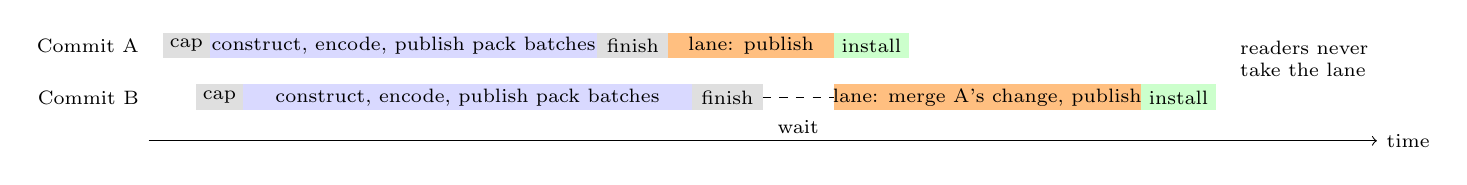
\begin{tikzpicture}[font=\scriptsize,x=0.6cm,y=0.55cm]
\draw[->] (0,0) -- (26,0) node[right]{time};
% Commit A
\node[anchor=east] at (0,2.2) {Commit A};
\fill[gray!25] (0.3,1.9) rectangle (1.3,2.5); \node at (0.8,2.2) {cap};
\fill[blue!15] (1.3,1.9) rectangle (9.5,2.5); \node at (5.4,2.2) {construct, encode, publish pack batches};
\fill[gray!25] (9.5,1.9) rectangle (11,2.5); \node at (10.25,2.2) {finish};
\fill[orange!50] (11,1.9) rectangle (14.5,2.5); \node at (12.75,2.2) {lane: publish};
\fill[green!20] (14.5,1.9) rectangle (16.1,2.5); \node at (15.3,2.2) {install};
% Commit B
\node[anchor=east] at (0,1.0) {Commit B};
\fill[gray!25] (1,0.7) rectangle (2,1.3); \node at (1.5,1.0) {cap};
\fill[blue!15] (2,0.7) rectangle (11.5,1.3); \node at (6.75,1.0) {construct, encode, publish pack batches};
\fill[gray!25] (11.5,0.7) rectangle (13,1.3); \node at (12.25,1.0) {finish};
\draw[dashed] (13,1.0) -- (14.5,1.0); \node[below] at (13.75,0.7) {wait};
\fill[orange!50] (14.5,0.7) rectangle (21,1.3); \node at (17.75,1.0) {lane: merge A's change, publish};
\fill[green!20] (21,0.7) rectangle (22.6,1.3); \node at (21.8,1.0) {install};
\node[anchor=west,align=left] at (22.9,1.9) {readers never\\take the lane};
\end{tikzpicture}
\caption{Two concurrent Commits on one Branch. Construction, compression and pack
batches overlap; only the lane serializes, and B merges only the change A published.}
\label{fig:twocommits}
\end{figure}

\paragraph{Read path.} A read that misses the kernel page cache (1) arrives as a FUSE
request of at most 128\,KiB, with one background request outstanding; (2) runs one
overlay job under the \ws{} lock that decides locally written bytes; (3) reads inherited
bytes \emph{outside} that lock from the shared object cache; (4) on a miss, issues one
batched Store demand, plus 8\,MiB of read-ahead for sequential streams (at most 16\,MiB
held per reader); and (5) decodes delta bases and zstd frames through a 2\,MiB pack
cache, re-hashing every object against its identifier. Mount reads only the root object.
Per-request round trips and decoding, not history depth, dominate read cost.

\paragraph{Lifecycles and custody.} A Sandbox lives from creation until it is explicitly
closed or its machine stops. A \ws{} is mounted, serves any number of processes and
Commits, and is unmounted; unmount refuses uncommitted changes unless told to discard
them. A Commit ends \texttt{Committed} (possibly after merging a moved head),
\texttt{UpToDate}, \texttt{Conflict} (marker blocks become the \ws{}'s local base and the
next Commit is refused while complete markers remain), or uncertain. Every hop makes one
attempt; a lost reply is reported as unknown and its custody (published outcome,
captured reader, operation intent) is retained until inspected. Committed history
survives a daemon or Sandbox loss, which loses only the disposable overlays. Under the
only permitted SQLite profile (WAL, \texttt{synchronous=OFF}) the Store survives process
termination, but a kernel or VM crash can lose or damage it.

% ---------------------------------------------------------------------------
\section{Committed State: Objects, Trees and Packs}
\label{app:objects}

All committed state of a Store lives in one SQLite file or PostgreSQL schema as two kinds
of data: immutable, content-addressed \emph{objects} that encode filesystem trees, and a
small set of mutable \emph{history} rows that name tree roots.

\paragraph{Objects.} Every object is a canonical byte string in a fixed envelope
(Table~\ref{tab:layouts}). Its identifier is
$\mathrm{BLAKE3}(\texttt{"layerfs/object/v2\textbackslash 0"} \,\|\, \text{canonical
bytes})$, 32 bytes. The value begins with an 8-byte role magic, so equal payload bytes
under different roles have different identifiers. Thirteen roles exist: whole file,
chunk, extent leaf and branch, file state, inode leaf and branch, directory leaf and
branch, filesystem root, attribute leaf and branch, and symlink. Identity-bearing integers
are big-endian. Decoders refuse padding, trailing bytes, nonzero flags, unknown versions
and unsorted rows rather than repairing them, so each logical value has exactly one
encoding, and references are always derived from the bytes, never supplied by a caller.

\begin{table}[h]
\centering
\small
\begin{tabular}{l p{0.7\linewidth}}
\toprule
Structure & Layout (bytes) \\
\midrule
Envelope (13) & \texttt{"LFSO"} [0:4] $\cdot$ kind \texttt{0x01} [4] $\cdot$ payload\_len u32 [5:9] $=$ value\_len$+4$ $\cdot$ value\_len u32 [9:13] $\cdot$ value \\
Tree-page header (31) & magic [0:8] $\cdot$ version u16 $\cdot$ role $\cdot$ level $\cdot$ flags$=0$ $\cdot$ count u16 $\cdot$ two subtree totals u64 \\
Whole file & \texttt{"LFS5SML\textbackslash 0"} $\cdot$ version u16 $\cdot$ payload (canonical $=$ raw $+$ 23) \\
Chunk & \texttt{"LFS4CHK\textbackslash 0"} $\cdot$ payload $\leq$ 32,768 \\
File state (93) & \texttt{"LFS4MAP\textbackslash 0"} $\cdot$ version $\cdot$ length u64 $\cdot$ extents u64 $\cdot$ level $\cdot$ profile id (32) $\cdot$ mapping root (32) \\
Extent leaf entry (40) & chunk id (32) $\cdot$ offset into chunk u32 $\cdot$ length u32 \\
Extent branch entry (48) & cumulative end bytes u64 $\cdot$ cumulative end extents u64 $\cdot$ child id (32) \\
Inode value (73) & kind (bit 7 $=$ inline) $\cdot$ link count u64 $\cdot$ content root (32) $\cdot$ \{attribute root (32) $|$ mode u32 $\cdot$ mtime s i64 $\cdot$ ns u32 $\cdot$ 16 zero\} \\
Filesystem root (116) & \texttt{"LFS6FSR\textbackslash 0"} $\cdot$ version $\cdot$ role $\cdot$ profile id (32) $\cdot$ scope id (32) $\cdot$ root serial u64 $\cdot$ inode-table root (32) \\
\bottomrule
\end{tabular}
\caption{Canonical byte layouts.}
\label{tab:layouts}
\end{table}

\paragraph{Trees.} A filesystem root names an inode table: a B$^+$-tree keyed by 64-bit
serial whose leaves hold 50--100 rows of (serial, 73-byte inode value) and whose
branches hold 64--127 (maximum serial, child) rows. A directory's content root is its own
B$^+$-tree from raw-byte name to serial; a name binds a serial, never an object, so a
hard link is two names for one serial. Tree pages are at most 8,192 bytes, and directory
and attribute pages are at least 40\% full except at the root. A regular file below the
cutoff (128\,KiB by default) is one whole-file object; a larger file is a file state over
an extent B$^+$-tree of 64--128 entries per page whose leaves map logical ranges to
\emph{slices}---(chunk, offset, length)---of content-defined chunks
(Figure~\ref{fig:tree}). Slices let a localized edit keep the untouched parts of boundary
chunks, and cumulative totals in branch entries locate an offset with one binary search
per level. Holes are not special: a run of zeros is a sequence of identical all-zero
32\,KiB chunks whose identical mapping pages are shared by identity. Profile identities
hashed from the frozen chunking and page parameters are embedded in each file state and
root and checked on decode. Updates rewrite only root-to-change paths; every unread
subtree keeps its identity.

\begin{figure}[h]
\centering
\small
\begin{verbatim}
FilesystemRoot --> InodeLeaf (root page of the inode table)
                    1: Dir   --> DirectoryLeaf { "a.bin" -> 2, "b.txt" -> 3 }
                    2: File  --> FileState(len, extents, level 1, profile)
                    3: File  --> WholeFile "LFS5SML\0" | bytes
FileState --> ExtentBranch [(end0,n0,L0) (end1,n1,L1)]
                L0 ExtentLeaf [(C1,0,len1) (C2,0,len2) ...]      (64-128 entries)
                L1 ExtentLeaf [(C2,4096,len) (C9,0,len9) ...]    <- a slice of C2
                     |
                Chunk C1, C2, C9 ...   (shared across files, versions, Branches, projects)
\end{verbatim}
\caption{One directory and one chunked file.}
\label{fig:tree}
\end{figure}

\paragraph{Physical records.} Identity excludes physical form. Payload objects (whole
files and chunks) are stored as \texttt{FULL} (a zstd frame), \texttt{STORED} (raw bytes,
chosen by an incompressibility probe) or \texttt{PREFIX} (a zstd frame compressed against
one base object's payload, recording the 32-byte base identifier). Inode branches and
directory and extent pages may be stored as a COPY/INSERT program against a predecessor
page (\texttt{COPY} $=$ 0 $\cdot$ offset u32 $\cdot$ length u32; \texttt{INSERT} $=$ 1
$\cdot$ length u32 $\cdot$ bytes), kept only when strictly smaller. Inode leaves are
pooled: each 73-byte value is replaced by a 4-byte ordinal, and values live in
append-only, field-packed blocks of at most 4,000 bytes and 255 entries ending in a
CRC32C. Every read rebuilds canonical bytes, base first along a delta chain, and hashes
each element against its identifier.

\paragraph{Packs.} Records are grouped (at most 8,191 records and 64\,KiB per group) into
immutable packs of at most 256\,KiB in four lanes: ordinary (tree pages, optionally
zstd-compressed per group), chunk, whole file, and singleton for one record too large for
a pack. A pack is a 24-byte header (\texttt{"LFPACK"}, version, group count, used
length), a directory of group offsets, encoded and decoded lengths and codecs, and the
group bodies; its key is the SHA-256 of its sealed bytes. A locator row maps each object
identifier to (role, canonical length, pack, group, record).

\begin{table}[h]
\centering
\small
\begin{tabular}{p{0.08\linewidth} p{0.24\linewidth} p{0.40\linewidth} p{0.18\linewidth}}
\toprule
Group & Table & Key $\rightarrow$ contents & Written by \\
\midrule
Physical & \texttt{pack} & pack id $\rightarrow$ SHA-256, length, body (update and delete refused by trigger) & object batches \\
 & \texttt{object\_location} & object id $\rightarrow$ role, canonical length, pack, group, record & object batches (insert if absent) \\
 & \texttt{inode\_value\_block} & first ordinal $\rightarrow$ $\leq$255 packed values $+$ CRC32C & object batches \\
 & \texttt{content\_signature} & ring slot $\rightarrow$ object id, 32-byte sketch & object batches (upsert) \\
 & \texttt{store\_policy}, \texttt{store\_totals} & cutoff, depth caps, next pack id and ordinal; byte totals & reservation, publication \\
History & \texttt{layer\_stack} & id $\rightarrow$ name, scope, profile, head Layer & init, \texttt{add\_layer} \\
 & \texttt{layer} & id $\rightarrow$ stack, parent, root, source Branch and Commit & \texttt{add\_layer} \\
 & \texttt{commit} & id $\rightarrow$ root, parent(s), base Layer, message, statistics, \texttt{.lww} decisions & publication lane \\
 & \texttt{branch} & id $\rightarrow$ name, base Layer, forked-from node, head Commit & fork, merge, lane \\
 & \texttt{scope\_allocator} & scope $\rightarrow$ serial high-water mark & serial reservation \\
Lineage & \texttt{layer\_lineage}, \texttt{commit\_lineage}, \ldots & heights, first-parent runs, absorption & with each Layer or Commit \\
Hints & \texttt{binding\_hint\_block}, \texttt{file\_digest} & name-binding hints; file-bytes digest $\rightarrow$ root & before the lane \\
\bottomrule
\end{tabular}
\caption{Store tables (SQLite; PostgreSQL is equivalent). Object batches run outside the
publication lane; only Commit insertion and head moves run inside it.}
\label{tab:schema}
\end{table}

\paragraph{History and invariants.} History identifiers are domain-separated BLAKE3
digests with a one-byte kind tag; a Commit identifier covers its root, parents, base
Layer and message but not its timestamp. Lineage tables record each Commit's
first-parent run and depth, so ancestry queries walk run segments rather than individual
Commits. The Store maintains six invariants: (i) every read authenticates; (ii) one
encoding per value; (iii) references are derived from bytes; (iv) packs, locators and
value blocks are append-only; (v) pack identifiers and inode serials are never reused;
(vi) Commits and Layers are immutable, and only Branch and stack heads move, by
expected-head checks. (Mutable rows besides heads are counters, the similarity ring and
the file-digest hint table.)

% ---------------------------------------------------------------------------
\section{Workspace Overlay and Request Path}
\label{app:overlay}

\paragraph{Overlay database.} Each mounted \ws{} owns one SQLite file created by a byte
copy of a schema-only template built at daemon start; mount therefore costs a fixed-size
file copy and one root-object read, independent of the tree. The file runs a disposable
profile (\texttt{journal\_mode=MEMORY}, \texttt{synchronous=OFF},
\texttt{locking\_mode=EXCLUSIVE}, 4\,KiB pages, no mmap, \texttt{busy\_timeout=0}) and
holds only changes (Table~\ref{tab:overlay}). All tables are \texttt{STRICT}; all except
the payload table and two single-key tables are \texttt{WITHOUT ROWID}. \texttt{fs\_data}
keeps a rowid so live runs can be overwritten in place with incremental blob I/O.

\begin{table}[h]
\centering
\small
\begin{tabular}{p{0.30\linewidth} p{0.62\linewidth}}
\toprule
Table & Rows \\
\midrule
\texttt{fs\_inode(inode, generation)} & One row per changed inode per generation: size, mode, mtime, kind, \texttt{inherited\_cutoff} \\
\texttt{fs\_entry(parent, name, generation)} & One row per changed name; a NULL inode is a whiteout \\
\texttt{fs\_data} & File bytes as 4\,KiB cells with a per-byte validity mask, or dense runs of whole cells inside one aligned 32\,KiB slot \\
\texttt{fs\_data\_ref} & \emph{Reference pieces}: ranges declared equal to committed bytes of a content root; no bytes stored \\
\texttt{fs\_truncate} & A shrink ``staircase'' so stale cells can be identified by epoch \\
\texttt{fs\_predecessor} & The file a rename replaced; an advisory delta base for the next Commit \\
\texttt{fs\_digest}, \texttt{cleanup\_task} & Append-only BLAKE3 digests; the reclamation queue \\
\bottomrule
\end{tabular}
\caption{Overlay schema (selected tables).}
\label{tab:overlay}
\end{table}

\paragraph{Layered view.} A \ws{}'s view is the committed base root plus overlay rows
with $\mathit{installed} < \mathit{generation} \leq \mathit{active}$. Each inode row
carries an \texttt{inherited\_cutoff}: bytes below it not written in that generation fall
through to the next lower layer and finally to the base file. Reads compose at most four
local layers newest-first and return the locally decided bytes, an \emph{inherited}
bitmask with one covering span, and reference ranges; the request then reads the span
and ranges from the immutable Store \emph{after} releasing the \ws{} lock.

\begin{figure}[h]
\centering
\resizebox{\linewidth}{!}{% Layered view of one file and the generation counters. Input by appendix.tex.
\begin{tikzpicture}[font=\scriptsize, x=1cm, y=1cm,
  cell/.style={draw, fill=orange!55, minimum height=0.42cm, inner sep=0},
  ref/.style={draw, pattern=north east lines, pattern color=blue!60, minimum height=0.42cm},
  ext/.style={draw, fill=gray!18, minimum height=0.42cm, inner sep=0},
  lbl/.style={anchor=east, align=right, font=\scriptsize},
  ar/.style={-{Stealth[length=4pt]}, thick}]
% ---------------- panel (a)
\node[font=\scriptsize\bfseries, anchor=west] at (-2.6,3.55) {(a) One file seen through the overlay};
% base file: committed extents (chunk slices)
\node[lbl] at (-0.15,0) {base file\\(committed root)};
\foreach \a/\b/\n in {0/1.6/c1, 1.6/2.9/c2, 2.9/4.7/c3, 4.7/5.9/c4, 5.9/7.6/c5, 7.6/9.0/c6}{
  \draw[fill=gray!18] (\a,-0.21) rectangle (\b,0.21); \node at ({(\a+\b)/2},0) {\n};}
% captured generation g
\node[lbl] at (-0.15,1.1) {generation $g$\\(captured)};
\draw[dotted] (0,0.89) rectangle (9.0,1.31);
\draw[fill=orange!55] (2.0,0.89) rectangle (2.25,1.31);
\draw[pattern=north east lines, pattern color=blue!60] (5.0,0.89) rectangle (6.6,1.31);
\node[font=\scriptsize, above] at (5.8,1.31) {reference piece};
\node[font=\scriptsize, above] at (2.12,1.31) {cell};
% active generation g+1, after a truncate and re-extension
\node[lbl] at (-0.15,2.2) {generation $g{+}1$\\(active)};
\draw[dotted] (0,1.99) rectangle (8.2,2.41);
\draw[fill=orange!55] (3.3,1.99) rectangle (4.1,2.41);
\node[font=\scriptsize, above] at (3.7,2.41) {32\,KiB run};
\draw[very thick, red!70!black] (7.0,1.85) -- (7.0,2.55);
\node[font=\scriptsize, red!70!black, above] at (7.0,2.55) {cutoff};
\fill[white] (7.0,1.99) rectangle (8.2,2.41);
\draw[dotted] (7.0,1.99) rectangle (8.2,2.41);
\node[font=\scriptsize] at (7.6,2.2) {zeros};
% composed view
\node[lbl] at (-0.15,-1.2) {what READ\\returns};
\foreach \a/\b/\c in {0/2.0/gray!18, 2.0/2.25/orange!55, 2.25/3.3/gray!18, 3.3/4.1/orange!55, 4.1/5.0/gray!18, 7.0/8.2/white}{
  \draw[fill=\c] (\a,-1.41) rectangle (\b,-0.99);}
\draw[pattern=north east lines, pattern color=blue!60] (5.0,-1.41) rectangle (6.6,-0.99);
\draw[fill=gray!18] (6.6,-1.41) rectangle (7.0,-0.99);
\node[font=\scriptsize] at (7.6,-1.2) {zeros};
\draw[decorate, decoration={brace, amplitude=3pt, mirror}] (0,-1.5) -- (8.2,-1.5)
  node[midway, below=3pt, font=\scriptsize, align=center] {one job under the \ws{} lock decides orange and zero bytes;\\gray and hatched bytes are read from the Store after it is released};
\draw[ar] (9.45,2.3) -- node[right, align=left, font=\scriptsize] {newest\\first} (9.45,0.0);
% ---------------- panel (b)
\begin{scope}[xshift=10.5cm]
\node[font=\scriptsize\bfseries, anchor=west] at (-0.3,3.55) {(b) Generation counters};
\draw[->] (0,2.4) -- (5.0,2.4) node[right] {gen};
\foreach \x/\t in {0.8/installed, 2.3/captured, 3.8/active}{
  \draw (\x,2.3) -- (\x,2.5); \node[above, font=\scriptsize] at (\x,2.5) {\t};}
\node[align=left, anchor=north west, text width=5.2cm] at (-0.3,2.0) {
\textbf{Visible rows}: $\mathit{installed} < \mathit{gen} \leq \mathit{active}$.\\[2pt]
\textbf{Capture} (Commit start): seal \emph{active} as \emph{captured};
new writes go to $\mathit{active}{+}1$. No row is copied.\\[2pt]
\textbf{Construct}: read only the sealed generation, in pages of $\leq$1,024 rows.\\[2pt]
\textbf{Install} (after publish): base root $\gets$ new root;
$\mathit{installed} \gets \mathit{captured}$ in one SQL step.\\[2pt]
\textbf{Reclaim}: rows at or below the floor are deleted after the reply, in small steps.};
\end{scope}
\end{tikzpicture}
}
\caption{(a) A file seen through the overlay: two generations of rows over the committed file. A READ composes them newest first, deciding locally written and zero bytes under the \ws{} lock and reading inherited and referenced bytes from the Store after releasing it. (b) Capture and install move counters, not rows.}
\label{fig:overlayview}
\end{figure}

\paragraph{Request path.} All state of one \ws{} sits behind one mutex. A job holds it
for at most one transaction and performs no Store I/O; base facts a job lacks are
returned as \emph{needs}, read without the lock, and supplied to a second job that
decides over the then-current rows. Kernel lookup counts, open descriptors, directory
cookies and read windows live in in-memory maps that commit or roll back with the job's
SQL. Windows bound each job, not files: a FUSE WRITE carries at most 128\,KiB (the
negotiated \texttt{max\_write}; the 256\,KiB job window is the NFS transfer size), a read
at most 128\,KiB, a page of rows at most 1,024. Algorithms~\ref{alg:write}
and~\ref{alg:read} show WRITE and READ.

\begin{algorithm}[h]
\caption{FUSE WRITE$(s, \mathit{off}, d)$, $|d| \leq 128$\,KiB}
\label{alg:write}
\small
\begin{algorithmic}[1]
\State $\mathit{claims} \gets$ \Call{Recognize}{$s, \mathit{off}, d$} \Comment{optional, bounded, no lock}
\Loop
  \State lock($W$) \Comment{one job, at most one transaction}
  \State $o \gets$ newest row of $s$ with generation in $(\mathit{installed}, \mathit{active}]$, else base facts
  \If{$o$ unknown} unlock; fetch base inode of $s$ without the lock; \textbf{continue} \EndIf
  \State \textbf{begin}; if no row $(s, \mathit{active})$, insert one with cutoff $\gets o.\mathit{size}$
  \ForAll{32\,KiB slots overlapping $[\mathit{off}, \mathit{off}+|d|)$}
    \State whole cells: overwrite the live dense run in place, or replace it with one run
    \State partial cell: point read, merge, set validity bits \Comment{no base read}
  \EndFor
  \State cells in $\mathit{claims}$ $\rightarrow$ reference pieces (no bytes)
  \State size $\gets \max(o.\mathit{size}, \mathit{off}+|d|)$; revision $\mathrel{+}= 1$; \textbf{commit}; unlock
  \State reply $|d|$; \textbf{return}
\EndLoop
\end{algorithmic}
\end{algorithm}

\begin{algorithm}[h]
\caption{FUSE READ$(s, \mathit{off}, n)$, $n \leq 128$\,KiB}
\label{alg:read}
\small
\begin{algorithmic}[1]
\State lock($W$) \Comment{read-only job}
\State $L \gets$ newest $\leq 4$ rows of $s$ with generation in $(\mathit{installed}, \mathit{active}]$
\ForAll{$\ell \in L$, newest first}
  \State copy live cells and runs of $\ell$ into undecided bytes
  \State mark bytes covered by $\ell$'s reference pieces as reference ranges
  \State mark bytes $\geq \ell.\mathit{cutoff}$ below EOF decided (zero if unwritten)
\EndFor
\State $r \gets$ base root at this instant; unlock
\If{every byte decided} reply \EndIf
\State read the inherited span of the base file at $r$ and the reference ranges \Comment{outside the lock}
\State reply
\end{algorithmic}
\end{algorithm}

\paragraph{No copy-up.} The first write to a committed file inserts one inode row whose
cutoff is the base length and stores only the written cells; no base byte is read or
copied, and partially written cells keep unwritten bytes inherited through their masks.
A truncate edits at most one 32\,KiB row, adds one staircase step and lowers the cutoff.
Appends past the old length skip even the row-shape read. Renames, including directory
renames and rename-over, change at most four inode rows and two name rows and move no
bytes; a rename-over records the replaced file as a predecessor. Hard links share one
serial and hence one kernel inode.

\paragraph{Capture and install.} A Commit seals the active generation by an in-memory
state change: \emph{active} becomes \emph{captured} and new mutations go to
$\mathit{active}+1$; no row is copied. Capture waits until every earlier mutation's reply
has been attempted, and later mutations wait behind it, so the captured frontier is
finite. Construction reads only the sealed generation, in pages of at most 1,024 rows.
After publication, install is one SQL step that sets the new base root and raises the
floor to the captured generation, plus a pointer swap of the base view; no tree is
walked. Rows written after the capture remain on top of the view, because their cutoffs
were taken from the sealed layer that the new root reproduces. Rows of the retired
generation are deleted after the Commit replies, in steps of at most 14 cells or 64 rows.

\begin{table}[h]
\centering
\small
\begin{tabular}{p{0.20\linewidth} p{0.22\linewidth} p{0.24\linewidth} p{0.12\linewidth} p{0.10\linewidth}}
\toprule
Operation & Overlay cost & Base cost & In tree size & In file size \\
\midrule
Mount & fixed template copy & one root object & $O(1)$ & -- \\
LOOKUP, GETATTR & $O(\log R)$ & $O(\log D + \log N)$ pages if unchanged & logarithmic & $O(1)$ \\
READ $w$ & $O(w + L\log R)$ & $O(w) + O(\log F)$ mapping pages & $O(1)$ & logarithmic \\
WRITE $w$ & $O(w + \log R)$ & none & $O(1)$ & $O(1)$ \\
Truncate & one $\leq$32\,KiB row $+ O(\log h)$ & none & $O(1)$ & $O(1)$ \\
CREATE, UNLINK, RENAME, LINK & $\leq$4 inode $+$ $\leq$2 name rows & name facts & $O(1)$ rows & $O(1)$ \\
Capture, install & in memory / one SQL step & one root object & $O(1)$ & $O(1)$ \\
\bottomrule
\end{tabular}
\caption{Per-request cost. $R$ changed rows, $N$ inodes, $D$ directory entries, $F$ file
size, $L \leq 4$ layers, $h$ staircase height. Logarithmic base costs follow from the
B$^+$-tree layout.}
\label{tab:overlaycost}
\end{table}

\paragraph{Limits.} Kernel write-back caching is off, so each \texttt{write(2)} is a
synchronous FUSE WRITE published to the overlay, and dirty shared-mapping pages not yet
sent are outside a capture. FLUSH and FSYNC answer \texttt{ENOSYS} once: durability
exists only at Commit. Extended attributes, READDIRPLUS, remote locks, \texttt{fallocate}
and \texttt{copy\_file\_range} are not implemented. Per-\ws{} open state (lookups,
descriptors, readers) is the one resident structure without a cap.

% ---------------------------------------------------------------------------
\IfFileExists{appendix-pipeline.tex}{% Input by appendix.tex. Notes: notes/appendix/P-pipeline.md.
\section{From \texttt{write(2)} to Stored Bytes}
\label{app:pipeline}

\sys{} turns filesystem calls into Store objects in two phases. At write time it records
\emph{what changed}, cheaply and without reading committed data. At Commit time it turns
that record into the smallest set of new immutable objects it can find in bounded work.
This appendix follows one byte range through content addressing, chunking, deduplication,
compression and delta encoding. Measurements are the evaluation's single samples
(Section~\ref{sec:eval}); stored bytes are exact.

\begin{figure}[h]
\centering
\resizebox{\linewidth}{!}{% write(2) -> stored bytes pipeline. Input by appendix-pipeline.tex.
\begin{tikzpicture}[
  font=\scriptsize,
  box/.style={draw, rounded corners=2pt, align=center, inner sep=3pt, minimum height=0.95cm, fill=white},
  st/.style={box, fill=blue!7},
  ov/.style={box, fill=yellow!15},
  sv/.style={box, fill=green!10},
  ln/.style={box, fill=orange!35},
  side/.style={box, dashed, fill=gray!6},
  ar/.style={-{Stealth[length=4pt]}, thick},
  lane/.style={font=\scriptsize\bfseries, anchor=west, text=black!70},
  node distance=0.32cm and 0.38cm
]
% ---- row 1: write time
\node[lane] (l1) at (-0.2,0.95) {1\;\; Write time: per FUSE request, under the \ws{} lock, no Store I/O};
\node[box] (w) at (0.9,0) {\texttt{write(2)}\\$\leq$128\,KiB};
\node[ov, right=of w, text width=3.3cm] (cells) {Overlay rows\\4\,KiB cells $+$ validity mask\\or 32\,KiB dense runs};
\node[side, right=of cells, text width=3.2cm] (rec) {Recognition ($\geq$8\,KiB)\\whole committed chunks\\$\rightarrow$ reference pieces};
\node[side, right=of rec, text width=3.0cm] (pred) {\texttt{rename()} over a file\\$\rightarrow$ predecessor row};
\draw[ar] (w) -- (cells);
\draw[ar,dashed] (rec) -- (cells);
\draw[ar,dashed] (pred.south) |- ++(0,-0.35) -| ([xshift=4pt]cells.south);
% ---- row 2: commit, before the lane
\node[lane] (l2) at (2.3,-1.5) {2\;\; Commit, before the lane: one producer thread, work $\propto$ changes};
\node[st, text width=1.8cm] (cap) at (1.15,-2.55) {Capture\\generation flip\\(no row copy)};
\node[st, right=of cap, text width=2.5cm] (shape) {Shape pass\\gaps and windows\\$\propto$ rows written};
\node[st, right=of shape, text width=2.8cm] (edits) {Edit list\\$(\mathit{start}, \mathit{removed}, \mathit{repl})$\\retained vs new bytes};
\node[st, right=of edits, text width=3.6cm] (build) {$\geq$\,$T$: split, slice, CDC only the\\replacement (8/16/32\,KiB),\\rebuild join paths\\$<$\,$T$: one whole-file object};
\draw[ar] (cells.south) -- ++(0,-0.4) -| (cap.north);
\draw[ar] (cap) -- (shape);
\draw[ar] (shape) -- (edits);
\draw[ar] (edits) -- (build);
% ---- row 3: Save
\node[lane] (l3) at (2.3,-4.4) {3\;\; Save: per new object, parallel across Commits};
\node[sv, text width=2.0cm] (id) at (1.25,-5.4) {Identity\\BLAKE3 of\\canonical bytes};
\node[sv, right=of id, text width=1.9cm] (dedup) {Already\\located?\\$\rightarrow$ reuse};
\node[sv, right=of dedup, text width=2.4cm] (ind) {Independent record\\1\,KiB probe: STORED\\else zstd-3 FULL};
\node[sv, right=of ind, text width=4.2cm] (delta) {One delta trial: base from aligner,\\predecessor, same path or ring;\\PREFIX iff strictly smaller};
\node[sv, right=of delta, text width=1.75cm] (pack) {Packs\\$\leq$256\,KiB\\4 lanes};
\draw[ar] (build.south) -- ++(0,-0.35) -| (id.north);
\draw[ar] (id) -- (dedup);
\draw[ar] (dedup) -- node[above,font=\tiny]{new} (ind);
\draw[ar] (ind) -- (delta);
\draw[ar] (delta) -- (pack);
% ---- row 4: pages and lane
\node[side, text width=7.6cm, minimum height=0.6cm, anchor=west] (pages) at (0.2,-6.85) {Tree pages (inode, directory, extent): COPY/INSERT program\\against the page they replace, else stored whole};
\node[ln, text width=2.6cm, minimum height=0.6cm] (lane) at (pack |- pages) {Lane: locators,\\Commit, head};
\draw[ar] (pack) -- (lane);
\draw[ar, dashed] (pages.east) -- ++(0.4,0) |- ([yshift=-6pt]delta.south) -- ([yshift=0pt]delta.south);
\node[font=\tiny, anchor=east, align=right] at ([xshift=-4pt]lane.west) {the only serialized step;\\$O(1)$ in tree size, history, Branches};
\end{tikzpicture}
}
\caption{From \texttt{write(2)} to stored bytes. Row 1 runs per request without Store I/O; rows 2 and 3 run before the publication lane, in parallel across Commits; only the lane is serialized.}
\label{fig:pipeline}
\end{figure}

\paragraph{Write time: localized-edit capture.} Kernel write-back is off, so every
\texttt{write(2)} reaches the daemon and is published into the \ws{}'s overlay
(Appendix~\ref{app:overlay}) before it returns. Bytes are kept as 4\,KiB cells, whose
per-byte validity mask distinguishes a written zero from a hole, or as dense runs of up
to 32\,KiB. Holes cost no rows, a shrink is one staircase row, and a write never reads
the committed bytes it partly covers. Two kinds of provenance are kept beside the bytes.
A \emph{reference piece} says that a range equals bytes of a committed file: \emph{write
recognition} creates one when a write of at least 8\,KiB contains whole chunks the file
already had, as when a program rewrites a file in place, and stops after 1\,MiB of
unmatched bytes. A \emph{predecessor} row records that \texttt{rename()} put one file
over another, which is how editors, Git and package managers save.

\paragraph{Capture to edit list.} A Commit seals the overlay generation without copying
rows. For each changed file a first pass reads only row \emph{shapes}: an unchanged
region is one indexed gap, so the pass grows with rows written, not with file length. A
one-pass script turns the spans into an ordered edit list in result coordinates. Bytes
inherited from the file's own base, or reference pieces of it, are \emph{retained};
everything else is new. Overwrites, appends (one trailing insert), truncations (one
trailing delete), holes (zero runs) and shifted rewrites (pieces plus a small residue,
with up to 64\,KiB at each edge compared against the base and trimmed where equal) all
come out in this one form, and a rewrite that reproduces the base exactly returns the
base root.

\paragraph{Construction.} Content applies the edits to the stored extent tree
(Algorithm~\ref{alg:edit}): it splits extents at each boundary, drops the replaced
middle unread, chunks only the replacement, and rebuilds pages only on the join paths.
Unchanged extents keep their chunk identities, possibly as slices. A file the base did
not hold---a new path, a renamed-over temporary file, a recreated path---is built from
scratch; because chunking is content-defined, its unchanged chunks resynchronize and are
the same objects as before. \emph{Small files} below the per-Store cutoff (128\,KiB by
default; any power of two up to 1\,MiB) are single whole-file objects, rebuilt whole on
every edit, so their natural delta base is the previous version of the whole file.

\paragraph{Storage.} Each object's identity is the BLAKE3 hash of its canonical bytes,
so identical files, chunks, pages and subtrees are stored once across Commits, Branches
and projects. The Save reuses any object already located, then gives each new payload
one representation trial (Algorithm~\ref{alg:select}). The independent record is a
level-3 zstd frame, or raw when a 1\,KiB probe saves at most 1/32. At most one delta base
is tried, and the delta is kept only if strictly smaller. Bases come from filesystem
events rather than search: the edited version, the aligned old chunk, the renamed-over
file or the file previously at the same path; a similarity sketch is the fallback for
whole files only. Tree pages get COPY/INSERT programs against the page they replace.
Chains are bounded in depth and decode work, and a chain that reaches a bound is
re-based onto its root. Records are grouped into append-only 256\,KiB packs inside the
single Store database; the ordinary lane compresses tree-page groups with zstd level~1.

\paragraph{The codec is frozen deliberately.} An offline study of 9,386 files under
128\,KiB found zstd-6 4.4\% smaller than zstd-3 at 2.6\X{} the compression CPU, a
trained dictionary 14\% smaller but requiring a new frame format, and 256\,KiB group
compression 22\% smaller but forcing 256\,KiB of decoding to serve a 2\,KB file.
\sys{} keeps per-object, random-access records and spends its effort on base selection
and metadata instead. The cost is visible: per-chunk frames lose cross-chunk context, so
64\,MiB of synthetic text stores 1.25\X{} larger than a whole-file \texttt{zstd -3}.

\begin{table}[h]
\centering
\small
\begin{tabular}{p{0.24\linewidth} p{0.33\linewidth} p{0.35\linewidth}}
\toprule
Workload pattern & Absorbed by & Measured \\
\midrule
Copy of a 50\,MB tree & File-digest relink, content addressing & Copy Commit of 500\,MB: 15.9\,KB, no payload; 11.9\X{} over 10 copies \\
Small text edit in place & Whole-file PREFIX delta against the edited version & delta$+$zstd 32.1\X{} (100 files, 20 Commits of 1\% edits) \\
Rename-over save, small file & Predecessor recorded at \texttt{rename()} & 32.0\X{}; payload equal to in-place editing \\
Rename-over save, large file & Content addressing $+$ aligned chunk bases & Git index churn $-$80\% (1.46\,MB $\rightarrow$ 0.30\,MB) \\
New path per version & Same-path base, similarity ring & 30.1\X{} \\
100\,B overwrite, 500\,MiB file & Cell row, one edit, one new chunk & 153\,B payload, 5.9\,KB stored per Commit \\
100\,B insert shifting a 10\,MiB tail & Recognition $\rightarrow$ reference pieces & 153\,B payload, 4.0\,KB metadata per Commit \\
16\,KiB append, 5\,MiB file & Trailing insert, losing-base back-off & 17.0\,KB per Commit ($+$0.3\% payload) \\
Truncate 500\,MiB to 0 & Split and discard & 8.4\,KB, metadata only \\
500\,MiB of random data & Raw after probe & $+$0.11\% payload \\
64\,MiB of zeros & Zero runs, repeated pages & 76\,B payload, 684\,B metadata \\
SQLite page churn & In-place page edits, chunk deltas & 13.7\X{} raw$\div$stored (a Git pack is 2.3\X{} smaller) \\
Tiny files & Whole-file objects, pooled metadata & 0.91\X{}: Store larger than raw \\
20 projects in one Store & Store-wide content addressing & 16.7\X{} smaller than 20 Stores \\
\bottomrule
\end{tabular}
\caption{Which mechanism absorbs which workload pattern.}
\label{tab:patterns}
\end{table}

\paragraph{Example 1: a 100-byte overwrite in a 500\,MiB file.} The write produces one
cell row in the overlay (two if it crosses a 4\,KiB boundary) and reads nothing from the
Store; recognition is skipped below 8\,KiB. At Commit the shape pass finds one local
window between two inherited gaps and emits a single overwrite edit. The edit reads the
mapping pages on the path to that offset---about 27,000 extents in a three-level tree,
by calculation---and the one stored chunk under the range, finds that the bytes differ,
splits the chunk's extent into two slices, scans the 100 bytes into one new chunk, and
rebuilds only that leaf, its ancestors and the 93-byte file state. Each rebuilt page is
offered its predecessor as a COPY/INSERT base, and the old overlapping chunk is offered
as the new chunk's delta base (random data stays raw). The parent directory is
untouched, because directory entries bind inode serials rather than content. Over five
Commits each stored 153\,B of payload and 5.7\,KB of metadata; the Store grew 7.4\,KB per
Commit and a cold Commit took 28\,ms, against 524\,MB and 0.6\,s for a whole-file
copy-up overlay. The same edit on 10\,MiB and 100\,MiB files stores the same 153\,B; in a
unit test, a larger file adds one page read per tree level (3 pages at 8\,MB, 4 at
24\,MB, the same three payloads).

\paragraph{Example 2: a rename-over save of a small file.} An editor writes
\texttt{f.tmp} (a new inode, say 40\,KiB) and calls \texttt{rename(f.tmp, f)}. The overlay
stores the new bytes as dense runs, rebinds the name \texttt{f} to the new serial and
records the old serial as its predecessor; no Store I/O happens. At Commit the new file
has no base of its own, so it is built from scratch as one whole-file object, and the
old file's root is declared as an explicit delta base without being read. The Save tries
one zstd frame with the old version as prefix (the 256\,KiB window covers both) and keeps
it if smaller. The directory page that maps \texttt{f} gets a COPY/INSERT program against
the page it replaces. On 100 such files with 1\% line edits, 20 Commits stored about
613\,B per file version (32.0\X{}, against 32.1\X{} for in-place editing); on a smaller
suite of 25 files the rename-over and in-place payloads are byte-identical. For a large
file saved this way, such as Git's index, the new file is re-chunked in full, unchanged
chunks dedupe by identity, and the aligner offers each new chunk the old chunk at the
same position: index churn fell 80\%, with 110 of 120 chunks stored as deltas.

\paragraph{Costs.} Tiny files cost about 200\,B each beyond their bytes, so a Store of
2\,KB files is about 10\% larger than the raw data. Metadata is about two-thirds of a
typical small Commit; fitted per-operation costs are 414\,B per edit, 1,360\,B per new
file, 1,111\,B per delete and 464\,B per rename. New data is written twice, once to the
overlay and again to the Store, so a 500\,MiB random write commits more slowly than in a
copy-up overlay (1.36\,s against 1.0\,s cold). A large file saved under a new inode is
re-chunked in full: storage stays small, but CPU does not, because recognition covers
only same-inode writes. Edits fragment the mapping into slices with no defragmentation,
and equal bytes may then have different roots, which is why diff and merge compare
bytes. Nothing is garbage-collected or repacked: removing a 500\,MiB file frees nothing
until a collector exists.
}{}

% ---------------------------------------------------------------------------
\section{Algorithms}
\label{app:algorithms}

\subsection{Content-defined chunking}

\sys{} uses a FastCDC-style GEAR scanner~\cite{fastcdc} with minimum 8\,KiB, target
16\,KiB and maximum 32\,KiB, two bytes per step, and normalization level~2: the cut
probability per byte is $2^{-16}$ between 8 and 16\,KiB and $2^{-12}$ between 16 and
32\,KiB. The first 8\,KiB of each chunk are copied without hashing. Scanner state
(chunk buffer, hash, and a pending odd byte) persists across reads, so read-buffer
boundaries never move a cut. The profile (sizes, masks, seed and table) is digested into
every file state.

\emph{Zero runs.} For a run of zeros the scanner state repeats with period 32\,KiB. A hole
of length $\ell$ is handled as one 32\,KiB scan, a repeat count $n = \lfloor(\ell -
32\,\mathrm{KiB})/32\,\mathrm{KiB}\rfloor$ of one all-zero chunk, and the remainder; the
mapping builder emits \emph{one} uniform page of 128 identical entries to stand for every
full page and recurses on the next level. A hole of any length therefore costs
$O(32\,\mathrm{KiB})$ scanning plus $O(h \cdot 128)$ mapping work for tree height $h =
O(\log_{128}(\ell/32\,\mathrm{KiB}))$, and yields the same partition and root as
byte-by-byte scanning.

\subsection{Localized edits and the aligner}

Edits are $(\mathit{start}, \mathit{removed}, \mathit{replacement})$ in result
coordinates. Algorithm~\ref{alg:edit} applies them to a chunked file. The removed middle
is discarded unread; only replacement bytes are chunked, with a fresh scanner, so CDC
never resynchronizes across an edit boundary and the two boundary chunks become slices.
Each edit costs two splits and two concatenations, each touching $O(h)$ pages on one
root-to-boundary path. The cost is therefore independent of file size: the same
overwrite reads 3 mapping pages on an 8\,MB file and 4 on a 24\,MB file.

\begin{figure}[h]
\centering
\resizebox{0.82\linewidth}{!}{% Localized edit on a file's extent tree: path copying with slices. Input by appendix.tex.
\begin{tikzpicture}[font=\scriptsize,
  pg/.style={draw, rounded corners=1.5pt, minimum width=1.05cm, minimum height=0.48cm, inner sep=1pt, fill=gray!12},
  nw/.style={pg, fill=orange!45, very thick},
  ch/.style={draw, minimum height=0.42cm, inner sep=1pt, fill=gray!12},
  chn/.style={ch, fill=orange!45},
  e/.style={-{Stealth[length=3pt]}},
  en/.style={-{Stealth[length=3pt]}, orange!70!black, thick}]
% old version (gray) and new version (orange) share every page off the edit path
\node[pg] (s0) at (3.2,3.2) {FileState$_0$};
\node[nw] (s1) at (8.6,3.2) {FileState$_1$};
\node[pg] (r0) at (3.2,2.3) {root$_0$};
\node[nw] (r1) at (8.6,2.3) {root$_1$};
\node[pg] (b1) at (1.4,1.25) {branch $B_1$};
\node[pg] (b2) at (5.0,1.25) {branch $B_2$};
\node[nw] (b2n) at (9.4,1.25) {branch $B_2'$};
\foreach \i/\x in {1/0.2,2/1.9,3/3.6,4/5.6}{\node[pg] (l\i) at (\x,0.2) {leaf $L_\i$};}
\node[nw] (l3n) at (9.4,0.2) {leaf $L_3'$};
\draw[e] (s0) -- (r0); \draw[e] (r0) -- (b1); \draw[e] (r0) -- (b2);
\draw[e] (b1) -- (l1); \draw[e] (b1) -- (l2); \draw[e] (b2) -- (l3); \draw[e] (b2) -- (l4);
\draw[en] (s1) -- (r1); \draw[en] (r1) -- (b2n); \draw[en] (b2n) -- (l3n);
\draw[en] (r1.west) .. controls (6.5,2.2) and (3.0,1.9) .. (b1.north east);
\draw[en] (b2n.south west) .. controls (8.0,0.6) and (7.0,0.6) .. (l4.north east);
% chunks under L3 and L3'
\node[ch, minimum width=1.4cm] (k5) at (2.8,-0.95) {$c_5$};
\node[ch, minimum width=1.8cm] (k6) at (4.45,-0.95) {$c_6$};
\draw[e] (l3) -- (k5); \draw[e] (l3) -- (k6);
\node[chn, minimum width=0.55cm] (n) at (9.4,-0.95) {$n$};
\draw[en] (l3n.south) -- (n);
\draw[en] (l3n.west) to[out=185,in=50] (k6.north east);
% leaf entries
\node[draw, fill=white, anchor=north west, align=left, font=\scriptsize] at (6.7,-1.45) {
$L_3$:\; $(c_5, 0, |c_5|)\;\; (c_6, 0, |c_6|)$\\
$L_3'$:\; $(c_5, 0, |c_5|)\;\; (c_6, 0, a)\;\; (n, 0, 100)\;\; (c_6, a{+}100, |c_6|{-}a{-}100)$};
\draw[decorate, decoration={brace, amplitude=3pt, mirror}] (3.55,-1.25) -- (5.35,-1.25)
  node[midway, below=3pt, font=\scriptsize, align=center] {100\,B overwrite at offset $a$\\$c_6$ becomes two slices; not re-chunked};
% legend
\node[anchor=north west, align=left, font=\scriptsize] at (-1.3,-1.3) {gray: shared with version 0\\orange: new in this Commit};
\end{tikzpicture}
}
\caption{A 100\,B overwrite inside chunk $c_6$. The Commit writes only the orange path (leaf, branch, root, file state) and one 100\,B chunk $n$; $c_6$ is kept as two slices, and every other page and chunk is shared with version 0.}
\label{fig:edittree}
\end{figure}

\begin{algorithm}[h]
\caption{Apply localized edits to a chunked file}
\label{alg:edit}
\small
\begin{algorithmic}[1]
\Function{ReplaceChunked}{$\mathit{base}, E$}
  \State $T \gets$ mapping tree of $\mathit{base}$; $A \gets$ \Call{Aligner}{$\mathit{base}$}; $\mathit{shift} \gets 0$
  \ForAll{$e \in E$ in ascending order}
    \State $(L, R_0) \gets$ \Call{Split}{$T, e.\mathit{start}$}; $(X, R) \gets$ \Call{Split}{$R_0, e.\mathit{removed}$} \Comment{$X$ discarded unread}
    \State $M \gets \bot$
    \If{$e.\mathit{replacement} > 0$}
      \State $A$.anchor($e.\mathit{start}$, $e.\mathit{start} - \mathit{shift}$)
      \State $M \gets$ CDC-build(replacement bytes, delta hint $\gets A$.offer)
    \EndIf
    \State $\mathit{shift} \mathrel{+}= e.\mathit{replacement} - e.\mathit{removed}$
    \State $T \gets \textsc{Concat}(\textsc{Concat}(L, M), R)$ \Comment{rebuild join paths only}
  \EndFor
  \State \Return new file state over $T$
\EndFunction
\Statex
\Function{Offer}{$\mathit{start}, \mathit{len}, \mathit{id}$} \Comment{aligner: delta base for a new chunk}
  \State $[f, t) \gets$ old byte range $[\mathit{start} - \mathit{shift}, \mathit{start} - \mathit{shift} + \mathit{len})$
  \If{an old extent in the window has payload $\mathit{id}$}
    \State re-anchor $\mathit{shift}$ at it; \Return $\bot$ \Comment{unchanged chunk: exact reuse}
  \EndIf
  \State \Return the old chunk with the largest overlap with $[f, t)$, else the successor of the last anchor
\EndFunction
\end{algorithmic}
\end{algorithm}

\subsection{Choosing a representation}

Each new payload object first receives an independent record: \texttt{STORED} if a
1\,KiB zstd probe saves at most 1/32, else a level-3 zstd frame (falling back to
\texttt{STORED} if the frame is not smaller). Algorithm~\ref{alg:select} then makes at
most one delta trial. Candidates come from filesystem events first: the aligner for
edited files; for fresh files, the rename-over predecessor recorded by the overlay, else
the file the base held at the same path. Only whole files with no event-derived base
consult the similarity ring. $T$ is the Store's whole-file cutoff (128\,KiB by default).

\begin{algorithm}[h]
\caption{Representation selection for one payload object}
\label{alg:select}
\small
\begin{algorithmic}[1]
\Function{Select}{$\mathit{id}, \mathit{raw}, \mathit{role}, \mathit{advisory}$}
  \State $\mathit{full} \gets$ \Call{Independent}{$\mathit{raw}$}; $\mathit{cap} \gets 16$ (whole file) or $8$ (chunk)
  \If{$\mathit{role} = $ chunk}
    \State $c \gets \mathit{advisory}[0]$; \textbf{if} $c$ is in back-off \textbf{then return} $\mathit{full}$
  \Else
    \State $c \gets$ first eligible advisory base, else \Call{Ring.Propose}{$\mathit{id}$, signature($\mathit{raw}$)}
  \EndIf
  \If{$c = \bot$ or ineligible} \Return $\mathit{full}$ \EndIf
  \If{$c$ is at the depth cap or its chain exceeds the budgets}
    \State $c \gets$ root of $c$'s chain \Comment{re-base: new object lands at depth 1}
  \EndIf
  \If{$\Sigma$decoded$(c) + |\mathit{raw}| > 4T$ or $\Sigma$encoded$(c) + |\mathit{raw}| > 2T$} \Return $\mathit{full}$ \EndIf
  \State $b \gets$ \Call{Acquire}{$c$} \Comment{authenticated, charged to the budgets}
  \State $p \gets$ zstd-3($\mathit{raw}$, prefix $=$ payload($b$)) \Comment{exactly one trial}
  \If{$\mathit{role} = $ chunk} record a win for $c$ iff $p$ saves at least $|\mathit{full}|/8$ \EndIf
  \If{$|p| < |\mathit{full}|$} \Return \texttt{PREFIX}$(c, p)$ \Comment{strictly smaller; ties keep FULL} \EndIf
  \State \Return $\mathit{full}$
\EndFunction
\end{algorithmic}
\end{algorithm}

\emph{Back-off.} A chunk base whose trials keep losing---for example the old last chunk
offered to every appended chunk---is skipped starting at the eighth consecutive loss,
with the skip doubling per further loss up to $2^{16}$; a win forgets it. On a 500\,MiB
append this reduced delta trials from 26,966 to 22 with identical stored bytes.

\emph{Similarity ring.} A whole file's signature is the bottom-8 of a splitmix-finalized
Rabin--Karp hash over 16-byte windows~\cite{broder}, folded to 32 bits. The ring holds
8,192 slots and a 65,536-entry reference table (704\,KiB in total, persisted with the
Store). A proposal requires at least two of the eight hashes to overlap and prefers the
newest entry, so the latest version of a lineage is proposed. Only objects that found no
other base, or won against a ring-proposed base admitted before the current Save, enter
the ring. A false proposal costs one trial and is harmless under the strictly-smaller
rule.

\begin{figure}[h]
\centering
\resizebox{\linewidth}{!}{% Delta chains: depth cap and re-base; chunk back-off. Input by appendix.tex.
\begin{tikzpicture}[font=\scriptsize,
  ob/.style={draw, rounded corners=1.5pt, minimum width=0.85cm, minimum height=0.5cm, inner sep=1pt},
  full/.style={ob, fill=gray!25},
  pre/.style={ob, fill=blue!10},
  bk/.style={-{Stealth[length=3pt]}}]
\node[font=\scriptsize\bfseries, anchor=west] at (-0.5,1.75) {(a) Whole-file chain, cap 16: re-base instead of FULL};
\node[full] (v1) at (0,0) {$v_1$};
\node[pre] (v2) at (1.15,0) {$v_2$};
\node[pre] (v3) at (2.3,0) {$v_3$};
\node (dots) at (3.35,0) {$\cdots$};
\node[pre] (v16) at (4.4,0) {$v_{17}$};
\node[pre, fill=orange!45] (v17) at (6.4,0) {$v_{18}$};
\draw[bk] (v2) -- (v1); \draw[bk] (v3) -- (v2); \draw[bk] (dots) -- (v3); \draw[bk] (v16) -- (dots);
\draw[bk, orange!70!black, thick] (v17.north) to[out=160,in=20] node[above, font=\scriptsize]{re-based onto the chain root: depth 1} (v1.north);
\draw[bk, dashed, gray] (v17) -- node[below, font=\scriptsize, align=center]{would be\\depth 17} (v16);
\foreach \n/\d in {v1/0, v2/1, v3/2, v16/16, v17/1}{\node[font=\scriptsize, below=1pt of \n] {d=\d};}
\node[anchor=west, align=left, font=\scriptsize, text width=4.6cm] at (7.3,0.1) {Reading any object decodes at most cap$+1$ records, $\leq 4T$ decoded and $\leq 2T$ encoded bytes (512 / 256\,KiB). Re-base cost: $+$22.5\% mean decode; edit-Commit payload 290\,$\rightarrow$\,120\,KB.};
% (b) back-off
\begin{scope}[yshift=-2.1cm]
\node[font=\scriptsize\bfseries, anchor=west] at (-0.5,0.75) {(b) Chunk base back-off: appended chunks keep losing against the old last chunk};
\foreach \i in {1,...,8}{\draw[fill=red!35] ({(\i-1)*0.42},-0.2) rectangle ++(0.36,0.4);}
\node[font=\scriptsize, below] at (1.6,-0.25) {8 losing trials};
\foreach \x/\g in {3.6/1, 4.4/2, 5.6/4, 7.5/8}{
  \draw[fill=red!35] (\x,-0.2) rectangle ++(0.36,0.4);
  \node[font=\scriptsize, above] at ({\x-0.25*\g*0.3-0.1},0.2) {skip \g};}
\draw[gray, decorate, decoration={snake, amplitude=1pt, segment length=4pt}] (3.4,0) -- (3.6,0);
\draw[gray, decorate, decoration={snake, amplitude=1pt, segment length=4pt}] (3.96,0) -- (4.4,0);
\draw[gray, decorate, decoration={snake, amplitude=1pt, segment length=4pt}] (4.76,0) -- (5.6,0);
\draw[gray, decorate, decoration={snake, amplitude=1pt, segment length=4pt}] (5.96,0) -- (7.5,0);
\node at (8.3,0) {$\cdots\;2^{16}$};
\node[anchor=west, align=left, font=\scriptsize, text width=4.6cm] at (9.1,0) {Skipped chunks are stored FULL with no trial; a win resets the base. 500\,MiB append: 26,966 $\rightarrow$ 22 trials, identical stored bytes.};
\end{scope}
\end{tikzpicture}
}
\caption{Bounding delta work. (a) A whole-file object that would exceed the depth cap is delta-encoded against the chain root instead of being stored FULL. (b) A chunk base that keeps losing is skipped for exponentially growing gaps.}
\label{fig:deltachain}
\end{figure}

\subsection{Exact reuse and chain reads}

Objects reach storage in waves. Duplicate identifiers within a wave are compared byte for
byte. An identifier already located with the same role and canonical length is reused
without reading it back; integrity is deferred to the read path. Concurrent writers are
arbitrated by insert-if-absent locators, and a losing writer compares its bytes with the
winner's (a mismatch is a collision error). Reading an object resolves its delta chain
iteratively, rejects cycles and chains longer than the role's cap, enforces the decoded
and encoded budgets, reconstructs base first, and authenticates every element against
its identifier.

\subsection{Commit}

\begin{algorithm}[h]
\caption{Commit of a \ws{}}
\label{alg:commit}
\small
\begin{algorithmic}[1]
\Function{Commit}{$\mathit{ws}, \mathit{force}$}
  \If{another Commit of $\mathit{ws}$ is in flight} \Return \texttt{Busy} \EndIf
  \If{no dirty rows, no pending merge, and head and base unchanged since bind} \Return \texttt{UpToDate} \EndIf
  \State $G \gets$ \Call{Capture}{} \Comment{seal generation; no row copied}
  \State producer thread: construct changed inodes of $G$ over the immutable base $\rightarrow$ bounded queue (32 batches) $\rightarrow$ Save
  \State $\mathit{cur} \gets$ head; \textbf{if} $\mathit{cur}$ moved and $\neg\mathit{force}$ \textbf{then} $\mathit{root} \gets$ \Call{Merge}{bound root, candidate, $\mathit{cur}$}
  \State Save.finish; validate; prepare install
  \State \textbf{acquire publication lane}
  \State \quad $\mathit{now} \gets$ head; \textbf{if} $\mathit{now} \neq \mathit{cur}$ \textbf{then} $\mathit{root} \gets$ \Call{Merge}{$\mathit{cur}$, $\mathit{root}$, $\mathit{now}$} bounded to 1,024 inodes
  \State \quad \textbf{if} conflicted: install merged tree with markers as local base; publish nothing
  \State \quad \textbf{else} one write transaction: check expected head, insert Commit, advance Branch
  \State \textbf{release lane}; install new base; retire $G$ after the reply
\EndFunction
\end{algorithmic}
\end{algorithm}

Capture is $O(1)$. Construction and Save work is proportional to the captured changes.
The lane holds two head reads, an optional merge of at most 1,024 changed inodes with
byte comparison capped at 1\,MiB per file, and one write transaction, independent of
tree size, history length and Branch count.

\subsection{Three-way merge and byte equality}

Merge walks the inode-table difference between the base and one side in windows of 256
\emph{serials}, not paths, so a move on one side and an edit on the other compose (the
edit lands at the new path). For an inode changed on both sides it decides in order:
identical change or one side unchanged; a \texttt{/.lww} rule (newer modification time
wins, ours on a tie); a three-way line merge for text files up to 1\,MiB, with
Git-compatible marker blocks per conflicting hunk; ours for binaries (recorded as a
conflict); kept side wrapped in deletion markers for modify/delete; and a type conflict
otherwise. The inode-table difference reads only pages whose child identifiers differ.

Because localized edits make a file's root depend on its edit history, equal bytes can
have different roots, so ``same'' means same bytes. Byte equality walks both files'
extent cursors, skips extents that are identical in chunk, offset, length and position
without reading them, and compares only the remaining ranges in 256\,KiB windows with
early exit.

% ---------------------------------------------------------------------------
\IfFileExists{appendix-analysis.tex}{% Input by appendix.tex. Numbers: notes/E-evaluation.md, notes/appendix/P-pipeline.md.
\section{Time and Storage Analysis}
\label{app:analysis}

This appendix derives the time and storage cost of each operation from the structures
in Appendices~\ref{app:objects}--\ref{app:algorithms} and checks each bound against
measurements. Measurements come from the evaluation's campaigns
(Section~\ref{sec:eval}). Each is one sample unless noted; storage bytes are exact and
times are wall clock.

\paragraph{Notation.} A tree has $N$ inodes. A file has length $F$ and $C \approx
F/\bar{c}$ chunks, with measured mean chunk size $\bar{c} \approx 19$\,KB. Pages hold at
most $P = 8$\,KiB. The mapping tree of a file has height $h_F = \lceil \log_{64} C \rceil$
or less (3 for 500\,MiB), the inode table $h_N = O(\log_{50} N)$, and a directory with $D$
entries $h_D = O(\log D)$. A Commit captures a set $\Delta$ of changed inodes; changed
file $i$ received $w_i$ written bytes in $e_i$ separate edit runs. $T$ is the whole-file
cutoff (128\,KiB). $H$ is history length and $B$ the number of Branches.

\subsection{Time}

\begin{table}[h]
\centering
\small
\begin{tabular}{p{0.15\linewidth} p{0.30\linewidth} p{0.17\linewidth} p{0.28\linewidth}}
\toprule
Operation & Cost & Grows with & Measured (median) \\
\midrule
Mount & Template copy $+$ one root object & nothing & 17--43\,ms across machines \\
WRITE $w$ & $O(w + \log R)$ overlay rows; no Store I/O & $w$ & -- \\
READ $w$, cold & $O(w + h_F + h_N)$ pages; $\leq$ cap$+1$ records and $\leq 4T$ decoded per object & $w$; $\log F$, $\log N$ & 158\,MB/s large file; flat across history ($<$1\%) \\
Capture & Generation flip & nothing & -- \\
Commit, construction & $O\big(\sum_{i\in\Delta}(w_i + e_i h_F P) + |\Delta| h_N P\big)$ & changes only & 100\,B edit: 24.4 / 24.5 / 28.1\,ms at 10 / 100 / 500\,MiB \\
Commit, lane & 2 head reads, $\leq$1,024-inode merge, one transaction & nothing ($N$, $H$, $B$) & no-change Commit 15--21\,ms \\
Commit, new data & $O(w)$ chunking, hashing, zstd, packing & $w$ & 500\,MiB: 1.36\,s ($\approx$385\,MB/s) \\
Fork & One Branch row & nothing & -- \\
Merge & Pages whose child ids differ, windows of 256 serials; $\leq$1\,MiB byte compare per text file & changed serials & -- \\
Unmount & Drain, close, delete overlay file & open state & 14--31\,ms \\
\bottomrule
\end{tabular}
\caption{Time per operation. Mount, Commit and unmount times are CLI calls including
process launch and routing, which costs 26--54\,ms alone; the Commit times are cold.}
\label{tab:time}
\end{table}

\paragraph{File size does not enter a Commit.} A localized edit touches one
root-to-boundary path per edit boundary, so its construction cost is $O(w + e\,h_F P)$,
and $h_F$ grows by one level per 64--128$\times$ growth in $F$. A 50$\times$ increase in
file size (10 to 500\,MiB) raised the cold Commit of a 100\,B overwrite from 24.4 to
28.1\,ms; a copy-up overlay grew from 191 to 604\,ms over the same range, and its time is
$\Theta(F)$. In a unit test the same three-extent overwrite read 3 mapping pages on an
8\,MB file and 4 on a 24\,MB file.

\paragraph{Tree size, history and Branch count do not enter the lane.} The publication
lane holds two head reads, a merge bounded to 1,024 inodes, and one transaction that
inserts a Commit and advances one Branch head. None of these reads the tree beyond the
bounded merge, walks history or enumerates Branches. Work that does grow---capture of
large changes, construction, compression, pack writes, and a full merge when the head
has moved---runs before the lane, so concurrent Commits overlap in all of it
(Figure~\ref{fig:twocommits}).

\paragraph{Reads are bounded by structure, not history.} A cold read of $w$ bytes costs
$O(w)$ plus one root-to-leaf path in the inode table and in the file's mapping tree. Each
stored object resolves a delta chain of at most 16 (whole file) or 8 (chunk) records,
decoding at most $4T = 512$\,KiB and reading at most $2T = 256$\,KiB encoded; a chain
that would exceed these bounds is re-based onto its root when written. Reads of a 65\,MB
tree and of a 500\,MiB file were within 1\% of each other before and after 40 and 5
Commits of history. Large-file reads are slow in absolute terms (158\,MB/s cold against
943\,MB/s for ovnfs) because each 128\,KiB FUSE request is a round trip with one
background request outstanding; that is a kernel-route cost, not a history cost.

\paragraph{Per-call overhead.} For per-tool-call \ws{}s, the cost added to each call is
mount, Commit and unmount. On a Docker machine with a SQLite Store the clean tiny-workload
row measured 19.2, 16.0 and 16.8\,ms, about 52\,ms in all with process launch included.
Sandbox creation is separate and amortized over many calls: 0.39\,s median on Docker,
44--68\,ms natively on macOS and in Apple containers. File calls that need no process
pay neither, because they run in the SDK's process (Section~\ref{sec:filecalls}).

\paragraph{Where time is lost.} New data is written twice, once into the overlay and
again into the Store, so a 500\,MiB random write committed in 1.36\,s against 1.0\,s for
a copy-up overlay. FUSE publication of every \texttt{write(2)} makes write bandwidth a
small fraction of a kernel overlay's (Appendix~\ref{app:modal}). Large files saved under
a new inode are re-chunked in full at Commit.

\subsection{Storage}

\begin{figure}[h]
\centering
\resizebox{\linewidth}{!}{% Measured time and storage. Input by appendix-analysis.tex.
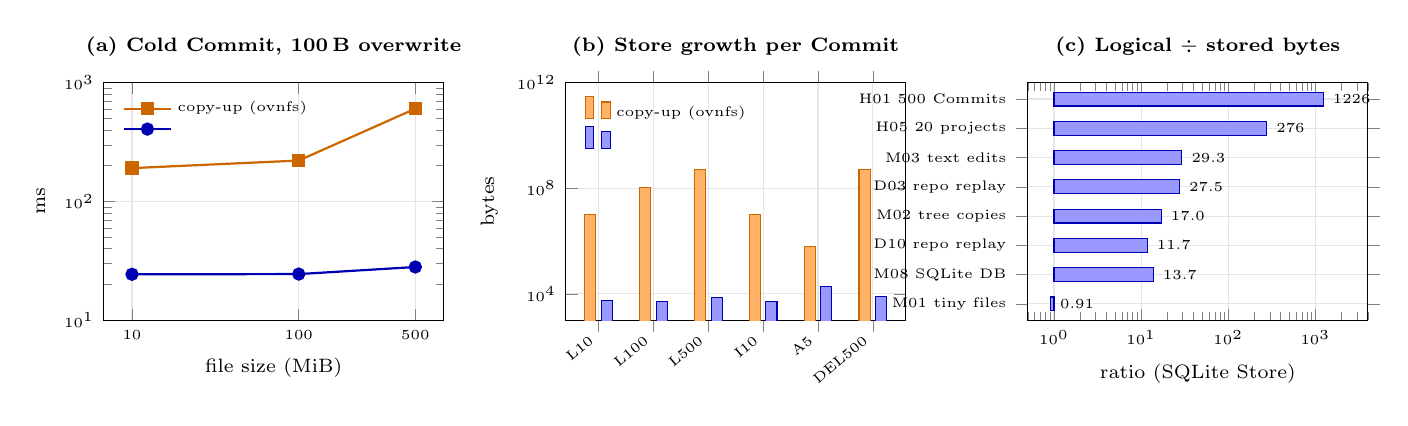
\begin{tikzpicture}
\begin{groupplot}[group style={group size=3 by 1, horizontal sep=1.55cm},
  width=5.9cm, height=4.6cm,
  tick label style={font=\tiny}, label style={font=\scriptsize}, title style={font=\scriptsize\bfseries},
  legend style={font=\tiny, draw=none, fill=none}, ymode=log, grid=major, grid style={gray!20}]
% (a) Commit time vs file size
\nextgroupplot[title={(a) Cold Commit, 100\,B overwrite}, xmode=log, xlabel={file size (MiB)}, ylabel={ms},
  xtick={10,100,500}, xticklabels={10,100,500}, ymin=10, ymax=1000, legend pos=north west]
\addplot[mark=square*, orange!80!black, thick] coordinates {(10,190.9) (100,221.1) (500,603.9)};
\addlegendentry{copy-up (ovnfs)}
\addplot[mark=*, blue!70!black, thick] coordinates {(10,24.4) (100,24.5) (500,28.1)};
\addlegendentry{\sys{}}
% (b) store growth per Commit
\nextgroupplot[title={(b) Store growth per Commit}, ybar, bar width=4pt, ylabel={bytes},
  symbolic x coords={L10,L100,L500,I10,A5,DEL500}, xtick=data, x tick label style={rotate=40, anchor=east, font=\tiny},
  ymin=1e3, ymax=1e12, legend pos=north west, enlarge x limits=0.12]
\addplot[fill=orange!60, draw=orange!80!black] coordinates {(L10,10.5e6) (L100,104.9e6) (L500,524.3e6) (I10,10.5e6) (A5,613e3) (DEL500,524.3e6)};
\addlegendentry{copy-up (ovnfs)}
\addplot[fill=blue!40, draw=blue!70!black] coordinates {(L10,5.5e3) (L100,5.3e3) (L500,7.4e3) (I10,5.3e3) (A5,18.4e3) (DEL500,8.2e3)};
\addlegendentry{\sys{}}
% (c) logical / stored
\nextgroupplot[title={(c) Logical $\div$ stored bytes}, xbar, bar width=5pt, xmode=log, ymode=normal,
  symbolic y coords={M01 tiny files,M08 SQLite DB,D10 repo replay,M02 tree copies,D03 repo replay,M03 text edits,H05 20 projects,H01 500 Commits},
  ytick=data, y tick label style={font=\tiny}, xmin=0.5, xmax=4000, xlabel={ratio (SQLite Store)},
  nodes near coords, nodes near coords style={font=\tiny, anchor=west}, point meta=explicit symbolic,
  enlarge y limits=0.08]
\addplot[fill=blue!40, draw=blue!70!black] coordinates {
 (0.91,M01 tiny files) [0.91] (13.73,M08 SQLite DB) [13.7] (11.71,D10 repo replay) [11.7] (16.97,M02 tree copies) [17.0]
 (27.48,D03 repo replay) [27.5] (29.27,M03 text edits) [29.3] (275.5,H05 20 projects) [276] (1225.9,H01 500 Commits) [1226]};
\end{groupplot}
\end{tikzpicture}
}
\caption{Measured time and storage. (a) Cold Commit time of a 100\,B overwrite is flat in file size for \sys{} and grows with it for a copy-up overlay. (b) Store growth per Commit for large-file edits (log scale; DEL500 truncates 500\,MiB). (c) Logical snapshot bytes over stored bytes across workloads; tiny files are the one case where the Store is larger than the data.}
\label{fig:charts}
\end{figure}

\paragraph{Cost of one change.} Store growth from a Commit is new payload plus new
metadata plus pack and locator overhead. Unchanged files, chunks, pages and subtrees
cost nothing, because identities are content hashes and updates rewrite only paths to
changes.
\begin{itemize}[leftmargin=*,nosep]
\item \emph{Payload.} A localized edit of $w$ bytes in a chunked file creates between
$\lceil w/32\,\mathrm{KiB}\rceil$ and $\lceil w/8\,\mathrm{KiB}\rceil + 1$ new chunks,
because only the replacement is chunked and boundary chunks become slices of existing
chunks. Payload is therefore at most $w$ plus per-record framing (or a smaller delta),
independent of $F$. A 100\,B random overwrite stored 153\,B of payload at 10, 100 and
500\,MiB. A small file ($< T$) is rewritten whole, so its payload is a delta against
the previous version, bounded by its compressed size.
\item \emph{Metadata.} A changed file rewrites at most $h_F$ mapping pages, a 93\,B file
state, $h_N$ inode-table pages and a 116\,B root; a name change also rewrites $h_D$
directory pages. Canonically this is $O((h_F + h_N + h_D)P)$, 17--26\,KB for a
mid-file overwrite of a large file. Each rewritten page is stored as a COPY/INSERT
program against the page it replaces, so 3.7--5.7\,KB is stored. Across mixed histories
a least-squares fit gives 414\,B per edit, 526\,B per append, 464\,B per rename,
1,111\,B per delete and 1,360\,B per new file.
\item \emph{Store overhead.} SQLite pages, locators and indexes add 1--20\% over the
stored records (1.01--1.20\X{}; PostgreSQL 1.05--1.39\X{}). Per object the floor is
about 200\,B, which dominates only for tiny files.
\end{itemize}

\begin{table}[h]
\centering
\small
\begin{tabular}{p{0.32\linewidth} p{0.20\linewidth} p{0.38\linewidth}}
\toprule
Change & Cost bound & Measured \\
\midrule
100\,B overwrite of a 500\,MiB file & $O(w + h_F P)$ & 7.4\,KB growth per Commit (copy-up overlay: 524.3\,MB) \\
16\,KiB append to a 5\,MiB file & $O(w)$ & 18.4\,KB per Commit (613\,KB) \\
Truncate 500\,MiB off a 1,000\,MiB file & $O(h_F P)$ & 8.2\,KB (524.3\,MB) \\
Remove a 500\,MiB file & $O(h_N P)$ & 24.6\,KB; frees nothing \\
Copy a 50\,MB tree 10 times & $O(\text{metadata})$ & 15.9\,KB per copy Commit, 0 payload \\
Fork a Branch & one row; first Commit pays its paths & 5.4\,KB per identical Branch \\
Second project in a shared Store & $O(\text{metadata})$ for shared content & 220\,KB per Init (first: 23.6\,MB) \\
Commit in a 65\,MB tree (5 mixed ops) & $O(\sum$ changes$)$ & 5.9\,KB growth per Commit over 500 Commits \\
\bottomrule
\end{tabular}
\caption{Store growth per change. Copy-up figures are ovnfs on the same host.}
\label{tab:storagechange}
\end{table}

\paragraph{Cost of a history.} Store size after $k$ Commits is the initial tree plus
the sum of per-change costs; it does not grow with the size of each snapshot. Over 500
Commits on a 65\,MB tree (32.5\,GB of logical snapshots) the Store reached 26.5\,MB:
23.6\,MB of initial tree plus 5.9\,KB per Commit, a ratio of 1,226\X{} between logical
and stored bytes. Table~\ref{tab:ksnap} compares the growth of $k$ snapshots in which
each snapshot changes $m$ files of size $F$ by $w$ bytes. Copy-up overlays and
whole-file snapshot images grow with $F$; block copy-on-write grows with the touched
blocks, but has no cross-file deduplication or deltas; \sys{} grows with $w$ plus a
logarithmic path. A fully repacked Git pack is the tightest point of reference---1.10 to
1.31\X{} smaller on the measured histories, because one global repack deltas across all
versions---but Git keeps no live mountable view and must repack to reach that size.

\begin{table}[h]
\centering
\small
\begin{tabular}{p{0.30\linewidth} p{0.27\linewidth} p{0.33\linewidth}}
\toprule
System & Growth for $k$ snapshots & Measured point \\
\midrule
Copy-up overlay; whole-file snapshot images & $k\,m\,F$ & 100\,B edits to 100\,MiB file: 1.15\,GB after 10 \\
Block copy-on-write (Btrfs, ImageFS-blk) & $k\,m\,\lceil w/b\rceil b$ $+$ metadata & 4\,KiB change to 512\,MiB file: about 36\,KiB (Btrfs; recovered report) \\
Git after full repack & $\approx k\,m\,\delta(w)$, after repack & 1.10--1.31\X{} smaller than \sys{} \\
\sys{} & $k\,(m(w + c\,h_F P') + h_N P')$ & same 10 edits: 106.3\,MB, of which 104.9\,MB is the initial file \\
\bottomrule
\end{tabular}
\caption{Growth over $k$ snapshots. $b$ is the block size, $\delta(w)$ a delta of $w$
bytes, and $P'$ the stored size of a page program.}
\label{tab:ksnap}
\end{table}

\paragraph{Trade-offs taken.} Several storage choices were made, or refused, on their
time cost, following the rule that a large speed loss is not traded for a small storage
gain (Table~\ref{tab:tradeoffs}).

\begin{table}[h]
\centering
\small
\begin{tabular}{p{0.30\linewidth} p{0.30\linewidth} p{0.30\linewidth}}
\toprule
Choice & Time effect & Storage effect \\
\midrule
Re-base at the chain bound & $+$22.5\% mean decode; max 520,575\,B $\leq$ 4$T$ budget & Edit Commit payload 290\,KB $\rightarrow$ 120\,KB \\
Losing-base back-off & 500\,MiB append: 26,966 $\rightarrow$ 22 trials, 7.9 $\rightarrow$ 5.5\,s & Identical bytes \\
Win saving $<$1/8 counts as loss & 100\,MiB log append 1,540 $\rightarrow$ 977\,ms & $+$1.04\% stored \\
zstd-3, not zstd-6 (refused) & zstd-6 costs 2.6\X{} compression CPU & zstd-6 would save 4.4\% \\
Per-object records, no group compression (refused) & Group: decode 256\,KiB to serve 2\,KB & Group would save 22\% \\
Per-chunk frames & Random-access reads & Text 1.25\X{} larger than whole-file zstd \\
No garbage collection or repack & No background work & Deleted data is retained \\
\bottomrule
\end{tabular}
\caption{Speed and storage trade-offs, from the design records.}
\label{tab:tradeoffs}
\end{table}
}{}

% ---------------------------------------------------------------------------
\section{Comparison with Image-FUSE and Overlayfs Sandboxes}
\label{app:modal}

Agent sandboxes commonly build their root filesystem from a lazily loaded, read-only
image and a writable copy-on-write layer. Modal's design is a well-documented example
with two generations~\cite{modalvmfs,modalimagefs,modallaunch}. \emph{ImageFS} serves
images through a FUSE server backed by a whole-file content-addressed cache spanning
memory, local SSD, zonal caches, a CDN and blob storage, with a kernel overlayfs upper on
XFS above it; whole-file copy-up in that arrangement can, in Modal's words, cost
gigabytes of overhead to write individual bytes. For VM sandboxes, Modal reports that
exposing this stack over virtio-fs made metadata-heavy work several times slower
(recursive \texttt{chown} from about 4\,s to over a minute) and replaced it with
\emph{ImageFS-blk}: the host synthesizes a sparse ext4 image, serves its blocks lazily
over virtio-blk, and records guest writes block by block in a per-VM sparse file with a
dirty bitmap, so the guest kernel owns all metadata~\cite{modalvmfs,modalvm}. Snapshots
are exposed as images that store the modified files, with an alpha memory snapshot that
also captures processes; filesystem snapshots expire after 30 days by default and cannot
be listed~\cite{modalsnap}. Table~\ref{tab:modal} compares the designs.

\begin{table}[h]
\centering
\small
\begin{tabular}{p{0.14\linewidth} p{0.24\linewidth} p{0.24\linewidth} p{0.26\linewidth}}
\toprule
& FUSE image $+$ overlayfs & Block image (ImageFS-blk) & \sys{} \\
\midrule
Lower layer & Read-only image, whole-file content addressing & Synthesized sparse ext4 image & Any committed root of any Branch \\
Lazy-load unit & Whole file; 32\,MB read-ahead & Block, mapped to file ranges & Tree page, whole file $<$128\,KiB, 8--32\,KiB chunk; authenticated \\
Write target & overlayfs upper on XFS & Per-VM sparse file, dirty bitmap & Per-\ws{} SQLite overlay \\
Copy-up unit & Whole file & One block & None: 4\,KiB cells; references for unchanged chunks \\
Metadata ops & Copy-up of lower files unless \texttt{metacopy} & In guest (\texttt{chown} $\approx$2\,\textmu s) & One overlay row; one FUSE round trip \\
Snapshot output & Image of modified files & Image of modified files (dirty bitmap) & Immutable Commit; chunk dedup and deltas \\
Snapshot cost & $\propto$ bytes of modified files & Not published & $\propto$ changed paths and bytes \\
Fork, history, merge & New sandbox from image; no history & Same & Fork is one row; diff, merge, blame \\
Distribution & Fleet-wide cache tiers & Fleet-wide cache tiers & One Store (one kernel, or PostgreSQL) \\
Steady-state I/O & Kernel page cache and overlayfs & Guest ext4 and page cache & FUSE; write-back off; 128\,KiB requests \\
POSIX coverage & Full & Full (Docker inside the VM) & No xattrs, FIFOs, locks, \texttt{fallocate} \\
\bottomrule
\end{tabular}
\caption{Image-based sandbox filesystems and \sys{}. Modal entries are taken from its
publications and documentation, not reproduced.}
\label{tab:modal}
\end{table}

\begin{figure}[h]
\centering
\resizebox{\linewidth}{!}{% What a 100-byte overwrite of a 500 MiB file costs in three designs. Input by appendix.tex.
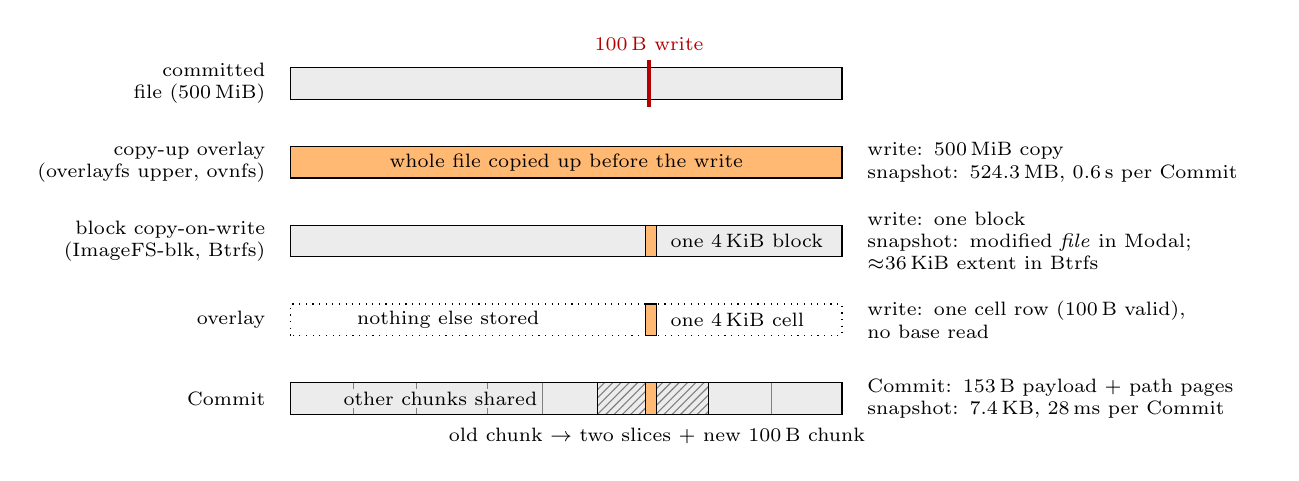
\begin{tikzpicture}[font=\scriptsize, x=1cm, y=1cm,
  lbl/.style={anchor=east, align=right, text width=2.9cm},
  note/.style={anchor=west, align=left, font=\scriptsize, text width=5.0cm}]
\def\W{7.0}
% lower layer, common
\node[lbl] at (-0.2,0) {committed file (500\,MiB)};
\draw[fill=gray!15] (0,-0.2) rectangle (\W,0.2);
\draw[red!70!black, very thick] (4.55,-0.3) -- (4.55,0.3);
\node[font=\scriptsize, red!70!black, above] at (4.55,0.3) {100\,B write};
% copy-up overlay
\node[lbl] at (-0.2,-1.0) {copy-up overlay\\(overlayfs upper, ovnfs)};
\draw[fill=orange!55] (0,-1.2) rectangle (\W,-0.8);
\node[font=\scriptsize] at (\W/2,-1.0) {whole file copied up before the write};
\node[note] at (\W+0.2,-1.0) {write: 500\,MiB copy\\snapshot: 524.3\,MB, 0.6\,s per Commit};
% block CoW
\node[lbl] at (-0.2,-2.0) {block copy-on-write\\(ImageFS-blk, Btrfs)};
\draw[fill=gray!15] (0,-2.2) rectangle (\W,-1.8);
\draw[fill=orange!55] (4.5,-2.2) rectangle (4.65,-1.8);
\node[font=\scriptsize, anchor=west] at (4.7,-2.0) {one 4\,KiB block};
\node[note] at (\W+0.2,-2.0) {write: one block\\snapshot: modified \emph{file} in Modal;\\$\approx$36\,KiB extent in Btrfs};
% LayerFS
\node[lbl] at (-0.2,-3.0) {\sys{} overlay};
\draw[dotted] (0,-3.2) rectangle (\W,-2.8);
\draw[fill=orange!55] (4.5,-3.2) rectangle (4.65,-2.8);
\node[font=\scriptsize, anchor=west] at (4.7,-3.0) {one 4\,KiB cell};
\node[font=\scriptsize] at (2.0,-3.0) {nothing else stored};
\node[note] at (\W+0.2,-3.0) {write: one cell row (100\,B valid),\\no base read};
\node[lbl] at (-0.2,-4.0) {\sys{} Commit};
\draw[fill=gray!15] (0,-4.2) rectangle (\W,-3.8);
\foreach \x in {0.8,1.6,2.5,3.2,3.9,5.3,6.1}{\draw[gray] (\x,-4.2) -- (\x,-3.8);}
\draw[fill=gray!15, pattern=north east lines, pattern color=gray] (3.9,-4.2) rectangle (5.3,-3.8);
\draw[fill=orange!55] (4.5,-4.2) rectangle (4.65,-3.8);
\node[font=\scriptsize, anchor=north] at (4.65,-4.25) {old chunk $\rightarrow$ two slices $+$ new 100\,B chunk};
\node[font=\scriptsize, fill=gray!15, inner sep=1pt] at (1.9,-4.0) {other chunks shared};
\node[note] at (\W+0.2,-4.0) {Commit: 153\,B payload $+$ path pages\\snapshot: 7.4\,KB, 28\,ms per Commit};
\end{tikzpicture}
}
\caption{What a 100\,B overwrite of a 500\,MiB file costs at write time and at snapshot time in each design. Copy-up and Commit figures are measured on one host; block copy-on-write figures are from Modal's description and a recovered Btrfs report.}
\label{fig:comparison}
\end{figure}

\paragraph{Where \sys{} wins.} The differences that matter for agents are in capture and
history. \sys{} never copies up: a 100\,B edit to a 500\,MiB file commits in 20--28\,ms
and adds 3--8\,KB, whereas a whole-file copy-up overlay (ovnfs, measured on the same
host) took about 0.6\,s and stored a full copy; across ten such edits to a 100\,MiB file
\sys{} stores 106\,MB against 1.15\,GB (Table~\ref{tab:ovnfs}). Against block-level
copy-on-write the write-time advantage largely disappears, but the snapshot difference
remains: Modal's documented snapshot unit is the modified file, so a database, a Git
pack or a build artifact touched by one byte is captured whole, and there is no
branch, merge, diff or history. In \sys{} every step is a Commit, forks are one row,
and unchanged chunks, pages and subtrees are shared across Commits, Branches and
projects.

\paragraph{Where \sys{} loses.} Raw I/O and coverage favor the image designs. Every
\sys{} write is a FUSE request published to SQLite before it returns, and the mount
negotiates 128\,KiB read-ahead with one background request. In an earlier three-way
measurement on the same host (a v1.0-era build, warm, one sample), kernel overlayfs
achieved 6\X{} the sequential-write and 75\X{} the 4\,KiB random-write bandwidth of
\sys{} and created small files 30\X{} faster; cold sequential reads of a 500\,MiB file
reach 158\,MB/s against 943\,MB/s for another FUSE overlay and about 2.5\,GiB/s that
Modal reports for ImageFS with 32\,MB read-ahead. ImageFS-blk performs metadata
operations entirely in the guest. \sys{} omits extended attributes, special files, locks
and \texttt{fallocate}, so Docker-in-sandbox, which Modal's VM runtime targets, cannot
run on a \ws{}. Modal distributes images across a fleet, while a \sys{} SQLite Store is
confined to one kernel.

\paragraph{Complementary, not competing.} The comparison is not a single ordering:
\sys{} is better at the operations that make sandbox state versioned---commit cost
proportional to change, sub-file copy-on-write, deduplication across snapshots, cheap
forks and history---and worse at steady-state throughput, POSIX coverage and fleet-scale
distribution. The designs also compose: a \sys{} \ws{} can run inside a VM whose block
device serves the operating system image, with \sys{} serving only the project. A fair
evaluation would run, on one native Linux host, \sys{}, a FUSE-image lower with an
overlayfs upper and whole-file snapshots, a block-level copy-on-write analog of
ImageFS-blk, and plain ext4, on (1) per-tool-call agent replays with a snapshot after
each mutating call, (2) small edits to 10\,MiB--1\,GiB files, a SQLite database and a
large Git repository, (3) Modal's own metadata and install workloads, (4) fork fan-out
to 64 views, and (5) 1,000 sequential snapshots, plus (6) a \sys{} ablation of
read-ahead, background requests and write-back caching that separates design cost from
tuning.

% ---------------------------------------------------------------------------
\IfFileExists{appendix-cli.tex}{% CLI reference appendix, generated from the 2.0 call table
% (origin/layerfs_v2_0_0 at 8cfb6e2734, api/crates/layerfs-api/src/<family>/<call>.rs).
% Source list: notes/cli-calls.md.
\section{Command-Line Interface}
\label{app:cli}

\sys{} 2.0 exposes one call table: 73 calls in ten families. The \texttt{layerfs}
command, the Node SDK and the Python SDK are all generated from it, so
\texttt{layerfs file write} on the command line is \texttt{layerfs.file.write} in the
SDKs, with the same positional arguments and options. Positionals run from the
outside in: owner, Branch, path or new name, other inputs, and an optional Commit
last. A project is named \texttt{<store>/<project>}. File content comes from standard
input or \texttt{--from}. Every call prints JSON, or text with \texttt{--text}; it exits
0 when done, 2 on a malformed command line and 125 when refused, with a structured
\texttt{\{code, message, detail\}} on standard error. Each call is attempted once and
never retried. Table~\ref{tab:cli} lists every call; five more commands exist only on
the command line (\texttt{help}, \texttt{--version}, \texttt{doctor},
\texttt{import-env} and \texttt{worker}).

{\footnotesize
\setlength{\LTpre}{4pt}\setlength{\LTpost}{0pt}
\begin{longtable}{@{}p{0.60\linewidth}@{\hspace{1em}}p{0.36\linewidth}@{}}
\caption{Every call of the \sys{} 2.0 command line, generated from the call table.
\texttt{[...]} marks an optional positional or option.}\label{tab:cli}\\
\toprule
Command & What it does \\
\midrule
\endfirsthead
\toprule
Command & What it does \\
\midrule
\endhead
\bottomrule
\endfoot
\multicolumn{2}{@{}l}{\textbf{Stores} (12)}\\*
{\raggedright\ttfamily layerfs store attach \textless{}name\textgreater{} \textless{}machine\textgreater{} [--url \textless{}url\textgreater{}] [--password \textless{}password\textgreater{}]} & Let a machine run Sandboxes of a PostgreSQL Store, after checking it reaches the server \\
{\raggedright\ttfamily layerfs store connect \textless{}name\textgreater{} \textless{}url\textgreater{} [--password \textless{}password\textgreater{}] [--synchronous-commit \textless{}synchronous-commit\textgreater{}]} & Attach a PostgreSQL database as a Store \\
{\raggedright\ttfamily layerfs store create \textless{}name\textgreater{}} & An empty sqlite Store on native \\
{\raggedright\ttfamily layerfs store detach \textless{}name\textgreater{} \textless{}machine\textgreater{}} & Stop a machine running Sandboxes of a PostgreSQL Store \\
{\raggedright\ttfamily layerfs store disconnect \textless{}name\textgreater{}} & Forget a PostgreSQL Store; its data stays \\
{\raggedright\ttfamily layerfs store get \textless{}name\textgreater{}} & A Store's record \\
{\raggedright\ttfamily layerfs store list} & Every Store, from the home's records \\
{\raggedright\ttfamily layerfs store pull \textless{}name\textgreater{} [--progress]} & Bring a sqlite Store from its machine to native \\
{\raggedright\ttfamily layerfs store push \textless{}name\textgreater{} \textless{}machine\textgreater{} [--progress]} & Send a sqlite Store from native to a machine \\
{\raggedright\ttfamily layerfs store remove \textless{}name\textgreater{}} & Delete a sqlite Store with every project in it \\
{\raggedright\ttfamily layerfs store stats \textless{}name\textgreater{}} & Store-wide publication and allocation counters \\
{\raggedright\ttfamily layerfs store status \textless{}name\textgreater{}} & A Store's live state \\
\addlinespace
\multicolumn{2}{@{}l}{\textbf{Projects} (6)}\\*
{\raggedright\ttfamily layerfs project export \textless{}project\textgreater{} \textless{}destination\textgreater{} [--branch \textless{}branch\textgreater{}] [--progress]} & Export a project's snapshot from its Store to a local folder \\
{\raggedright\ttfamily layerfs project get \textless{}project\textgreater{}} & A project's record: its Store, kind and machine \\
{\raggedright\ttfamily layerfs project init \textless{}project\textgreater{} \textless{}folder\textgreater{} [--timeout \textless{}timeout\textgreater{}] [--progress]} & Import a host folder as a new project into an existing Store \\
{\raggedright\ttfamily layerfs project list [\textless{}store\textgreater{}] [--page-size \textless{}page-size\textgreater{}] [--page-pos \textless{}page-pos\textgreater{}]} & Every project in the home, or one Store's \\
{\raggedright\ttfamily layerfs project remove \textless{}project\textgreater{}} & Remove one project from its Store \\
{\raggedright\ttfamily layerfs project stats \textless{}project\textgreater{} [\textless{}branch\textgreater{}] [\textless{}commit\textgreater{}]} & Entry counts of one pinned saved tree \\
\addlinespace
\multicolumn{2}{@{}l}{\textbf{Branches} (8)}\\*
{\raggedright\ttfamily layerfs branch commits \textless{}project\textgreater{} \textless{}branch\textgreater{} [--page \textless{}page\textgreater{}] [--page-size \textless{}page-size\textgreater{}] [--at-commit \textless{}at-commit\textgreater{}] [--include-storage]} & Saved branch commits or main publications, newest first \\
{\raggedright\ttfamily layerfs branch diff \textless{}project\textgreater{} \textless{}from-branch\textgreater{} \textless{}to-branch\textgreater{} [--paths-only] [--page-size \textless{}page-size\textgreater{}] [--page-pos \textless{}page-pos\textgreater{}] [--cursor \textless{}cursor\textgreater{}] [--page \textless{}page\textgreater{}] [--from-commit \textless{}from-commit\textgreater{}] [--to-commit \textless{}to-commit\textgreater{}] [--path-prefix \textless{}path-prefix\textgreater{}] [--include-attribution] [--continuation \textless{}continuation\textgreater{}]} & Files that differ between two Branches' heads \\
{\raggedright\ttfamily layerfs branch fork \textless{}project\textgreater{} \textless{}name\textgreater{} \textless{}from-branch\textgreater{} [\textless{}from-commit\textgreater{}]} & A new Branch from another Branch's head or Commit \\
{\raggedright\ttfamily layerfs branch get \textless{}project\textgreater{} \textless{}branch\textgreater{}} & One Branch and its head Commit \\
{\raggedright\ttfamily layerfs branch get-commit \textless{}project\textgreater{} \textless{}branch\textgreater{} \textless{}commit\textgreater{}} & One saved Commit or main publication \\
{\raggedright\ttfamily layerfs branch list \textless{}project\textgreater{} [--page-size \textless{}page-size\textgreater{}] [--page-pos \textless{}page-pos\textgreater{}] [--page \textless{}page\textgreater{}]} & A project's Branches \\
{\raggedright\ttfamily layerfs branch merge \textless{}project\textgreater{} \textless{}name\textgreater{} \textless{}a\textgreater{} \textless{}b\textgreater{} [--message \textless{}message\textgreater{}] [--units \textless{}units\textgreater{}]} & Merge two Branches into a new one \\
{\raggedright\ttfamily layerfs branch publish \textless{}project\textgreater{} \textless{}branch\textgreater{} [\textless{}commit\textgreater{}]} & A Branch's head or Commit as main's next Layer \\
\addlinespace
\multicolumn{2}{@{}l}{\textbf{Files (in-process; no Sandbox)} (15)}\\*
{\raggedright\ttfamily layerfs file apply \textless{}project\textgreater{} \textless{}branch\textgreater{} [--message \textless{}message\textgreater{}] [--from \textless{}file\textgreater{}]} & Apply a list of changes; one Commit \\
{\raggedright\ttfamily layerfs file blame \textless{}project\textgreater{} \textless{}branch\textgreater{} \textless{}path\textgreater{} [\textless{}commit\textgreater{}] [--from-line \textless{}from-line\textgreater{}] [--line-count \textless{}line-count\textgreater{}]} & The Commit of each line \\
{\raggedright\ttfamily layerfs file cp \textless{}project\textgreater{} \textless{}branch\textgreater{} \textless{}from-path\textgreater{} \textless{}to-path\textgreater{} [--message \textless{}message\textgreater{}]} & Copy a path; one Commit \\
{\raggedright\ttfamily layerfs file diff \textless{}project\textgreater{} \textless{}left-branch\textgreater{} \textless{}left-path\textgreater{} \textless{}right-branch\textgreater{} \textless{}right-path\textgreater{} [--left-commit \textless{}left-commit\textgreater{}] [--right-commit \textless{}right-commit\textgreater{}] [--include-attribution] [--allow-missing] [--page \textless{}page\textgreater{}] [--page-size \textless{}page-size\textgreater{}]} & The difference between two files \\
{\raggedright\ttfamily layerfs file edit \textless{}project\textgreater{} \textless{}branch\textgreater{} \textless{}path\textgreater{} [--old \textless{}old\textgreater{}] [--new \textless{}new\textgreater{}] [--message \textless{}message\textgreater{}]} & Replace one unique text in a file; one Commit \\
{\raggedright\ttfamily layerfs file glob \textless{}project\textgreater{} \textless{}branch\textgreater{} \textless{}path\textgreater{} \textless{}pattern\textgreater{} [\textless{}commit\textgreater{}] [--page-size \textless{}page-size\textgreater{}] [--page \textless{}page\textgreater{}] [--page-pos \textless{}page-pos\textgreater{}]} & Paths under path matching a glob \\
{\raggedright\ttfamily layerfs file grep \textless{}project\textgreater{} \textless{}branch\textgreater{} \textless{}path\textgreater{} \textless{}pattern\textgreater{} [\textless{}commit\textgreater{}] [--page-size \textless{}page-size\textgreater{}] [--page \textless{}page\textgreater{}] [--page-pos \textless{}page-pos\textgreater{}]} & Lines under path matching a regular expression \\
{\raggedright\ttfamily layerfs file list \textless{}project\textgreater{} \textless{}branch\textgreater{} \textless{}path\textgreater{} [\textless{}commit\textgreater{}] [--page-size \textless{}page-size\textgreater{}] [--page \textless{}page\textgreater{}] [--page-pos \textless{}page-pos\textgreater{}]} & A folder's entries \\
{\raggedright\ttfamily layerfs file mkdir \textless{}project\textgreater{} \textless{}branch\textgreater{} \textless{}path\textgreater{} [--message \textless{}message\textgreater{}] [--mode \textless{}mode\textgreater{}]} & Make a folder; one Commit \\
{\raggedright\ttfamily layerfs file mv \textless{}project\textgreater{} \textless{}branch\textgreater{} \textless{}from-path\textgreater{} \textless{}to-path\textgreater{} [--message \textless{}message\textgreater{}]} & Move a path; one Commit \\
{\raggedright\ttfamily layerfs file read \textless{}project\textgreater{} \textless{}branch\textgreater{} \textless{}path\textgreater{} [\textless{}commit\textgreater{}] [--start-line \textless{}start-line\textgreater{}] [--end-line \textless{}end-line\textgreater{}]} & Read a file \\
{\raggedright\ttfamily layerfs file revision \textless{}project\textgreater{} \textless{}branch\textgreater{} \textless{}path\textgreater{} [--at-commit \textless{}at-commit\textgreater{}] [--traversal \textless{}traversal\textgreater{}] [--page \textless{}page\textgreater{}] [--page-size \textless{}page-size\textgreater{}] [--continuation \textless{}continuation\textgreater{}]} & Saved changes to a literal path \\
{\raggedright\ttfamily layerfs file rm \textless{}project\textgreater{} \textless{}branch\textgreater{} \textless{}path\textgreater{} [--message \textless{}message\textgreater{}]} & Remove a path; one Commit \\
{\raggedright\ttfamily layerfs file stat \textless{}project\textgreater{} \textless{}branch\textgreater{} \textless{}path\textgreater{} [\textless{}commit\textgreater{}]} & A path's kind, size and mode \\
{\raggedright\ttfamily layerfs file write \textless{}project\textgreater{} \textless{}branch\textgreater{} \textless{}path\textgreater{} [--message \textless{}message\textgreater{}] [--mode \textless{}mode\textgreater{}] [--from \textless{}file\textgreater{}]} & Write a file; one Commit \\
\addlinespace
\multicolumn{2}{@{}l}{\textbf{Commits} (3)}\\*
{\raggedright\ttfamily layerfs commit diff \textless{}project\textgreater{} \textless{}from-commit\textgreater{} \textless{}to-commit\textgreater{} [--paths-only] [--page-size \textless{}page-size\textgreater{}] [--page-pos \textless{}page-pos\textgreater{}] [--cursor \textless{}cursor\textgreater{}]} & Files that differ between two Commits \\
{\raggedright\ttfamily layerfs commit get \textless{}project\textgreater{} \textless{}branch\textgreater{} \textless{}commit\textgreater{}} & One Commit of a Branch \\
{\raggedright\ttfamily layerfs commit list \textless{}project\textgreater{} \textless{}branch\textgreater{} [--page-size \textless{}page-size\textgreater{}] [--page-pos \textless{}page-pos\textgreater{}]} & A Branch's Commits, newest first \\
\addlinespace
\multicolumn{2}{@{}l}{\textbf{Sandboxes} (4)}\\*
{\raggedright\ttfamily layerfs sandbox close \textless{}name\textgreater{} [--force]} & Stop a Sandbox \\
{\raggedright\ttfamily layerfs sandbox create \textless{}project\textgreater{} \textless{}name\textgreater{} [\textless{}machine\textgreater{}] [--image \textless{}image\textgreater{}] [--progress]} & Start a named Sandbox of a project on a machine (default: its sqlite Store's, or native) \\
{\raggedright\ttfamily layerfs sandbox get \textless{}name\textgreater{} [--page-size \textless{}page-size\textgreater{}] [--page-pos \textless{}page-pos\textgreater{}]} & A Sandbox and its Workspaces \\
{\raggedright\ttfamily layerfs sandbox list [\textless{}project\textgreater{}] [--page-size \textless{}page-size\textgreater{}] [--page-pos \textless{}page-pos\textgreater{}]} & Every Sandbox in the home, or one project's \\
\addlinespace
\multicolumn{2}{@{}l}{\textbf{Workspaces} (6)}\\*
{\raggedright\ttfamily layerfs workspace commit \textless{}ws\textgreater{} [--message \textless{}message\textgreater{}] [--force]} & Commit a Workspace's changes to its Branch \\
{\raggedright\ttfamily layerfs workspace exec \textless{}ws\textgreater{} \textless{}command\textgreater{} [--message \textless{}message\textgreater{}] [--stream] [--exec-id \textless{}exec-id\textgreater{}] [--progress] [--events]} & Run one bash command in a Workspace \\
{\raggedright\ttfamily layerfs workspace exec-cancel \textless{}ws\textgreater{} \textless{}exec-id\textgreater{} [--grace-ms \textless{}grace-ms\textgreater{}]} & End a running command: SIGTERM, then SIGKILL after grace\_ms \\
{\raggedright\ttfamily layerfs workspace mount \textless{}sandbox\textgreater{} \textless{}branch\textgreater{} [--name \textless{}name\textgreater{}]} & Mount a Branch in a Sandbox \\
{\raggedright\ttfamily layerfs workspace status \textless{}ws\textgreater{}} & A Workspace's changes since its base \\
{\raggedright\ttfamily layerfs workspace unmount \textless{}ws\textgreater{} [--discard] [--force]} & End a Workspace \\
\addlinespace
\multicolumn{2}{@{}l}{\textbf{Machines} (12)}\\*
{\raggedright\ttfamily layerfs machine create \textless{}name\textgreater{} \textless{}platform\textgreater{} [--cpus \textless{}cpus\textgreater{}] [--memory \textless{}memory\textgreater{}] [--disk \textless{}disk\textgreater{}] [--image \textless{}image\textgreater{}] [--os-image \textless{}os-image\textgreater{}] [--progress]} & Create an enabled VM machine (apple-container, lima) \\
{\raggedright\ttfamily layerfs machine get \textless{}name\textgreater{}} & A machine's record \\
{\raggedright\ttfamily layerfs machine images \textless{}name\textgreater{}} & The Sandbox images a machine holds, and the host's Docker images it can copy \\
{\raggedright\ttfamily layerfs machine list} & Every machine, with what it supports \\
{\raggedright\ttfamily layerfs machine load \textless{}name\textgreater{} \textless{}image\textgreater{} [--progress]} & Copy an image from the host's Docker to a machine without creating a Sandbox \\
{\raggedright\ttfamily layerfs machine platforms} & The platforms this host and build support, and what each is missing \\
{\raggedright\ttfamily layerfs machine prune \textless{}name\textgreater{} [\textless{}image\textgreater{}] [--unused]} & Remove a Sandbox image from a machine, or every unused one \\
{\raggedright\ttfamily layerfs machine remove \textless{}name\textgreater{}} & Delete a VM machine and its disk; one of a removed platform is only forgotten \\
{\raggedright\ttfamily layerfs machine start \textless{}name\textgreater{} [--progress]} & Start a stopped machine and its worker; a running one answers at once \\
{\raggedright\ttfamily layerfs machine status \textless{}name\textgreater{}} & A machine's live state, free disk and tool version \\
{\raggedright\ttfamily layerfs machine stop \textless{}name\textgreater{} [--force]} & Stop a machine's worker and VM; its disks stay \\
{\raggedright\ttfamily layerfs machine update \textless{}name\textgreater{} [--cpus \textless{}cpus\textgreater{}] [--memory \textless{}memory\textgreater{}] [--image \textless{}image\textgreater{}] [--docker \textless{}docker\textgreater{}] [--wsl \textless{}wsl\textgreater{}] [--daemon \textless{}daemon\textgreater{}]} & Resize a VM, or set a built-in machine's image, Docker socket and daemon \\
\addlinespace
\multicolumn{2}{@{}l}{\textbf{Backups} (5)}\\*
{\raggedright\ttfamily layerfs backup connect \textless{}name\textgreater{} \textless{}url\textgreater{} [--key \textless{}key\textgreater{}] [--region \textless{}region\textgreater{}] [--part-size \textless{}part-size\textgreater{}]} & Connect an r2 or MinIO bucket \\
{\raggedright\ttfamily layerfs backup create \textless{}store\textgreater{} \textless{}bucket\textgreater{} [\textless{}file\textgreater{}] [--progress]} & Upload a sqlite Store to a bucket \\
{\raggedright\ttfamily layerfs backup disconnect \textless{}name\textgreater{}} & Forget a bucket and this home's links to it \\
{\raggedright\ttfamily layerfs backup list [\textless{}bucket\textgreater{}]} & Every Store file on the connected buckets \\
{\raggedright\ttfamily layerfs backup restore \textless{}store\textgreater{} \textless{}bucket\textgreater{} [\textless{}file\textgreater{}] [--progress]} & Download a backup as a sqlite Store on native \\
\addlinespace
\multicolumn{2}{@{}l}{\textbf{Call log} (2)}\\*
{\raggedright\ttfamily layerfs logs list [--op \textless{}op\textgreater{}] [--project \textless{}project\textgreater{}] [--client \textless{}client\textgreater{}] [--tag \textless{}tag\textgreater{}] [--outcome \textless{}outcome\textgreater{}] [--since \textless{}since\textgreater{}] [--cursor \textless{}cursor\textgreater{}] [--limit \textless{}limit\textgreater{}]} & The calls made against this home, newest first \\
{\raggedright\ttfamily layerfs logs reset} & Clear this home's call log \\
\addlinespace
\multicolumn{2}{@{}l}{\textbf{Command line only} (5)}\\*
{\raggedright\ttfamily layerfs help [\textless{}family\textgreater{} [\textless{}call\textgreater{}]]} & This list; \texttt{help --json} prints the call table \\
{\raggedright\ttfamily layerfs --version} & The build's version \\
{\raggedright\ttfamily layerfs doctor [--quick | --write-test] [--timeout \textless{}duration\textgreater{}]} & Report what is wrong in the home, changing nothing \\
{\raggedright\ttfamily layerfs import-env} & Write this environment's 1.1.0 settings as records, once \\
{\raggedright\ttfamily layerfs worker} & Serve this machine's worker (inside a machine) \\
\end{longtable}
}
}{}
